\documentclass[12pt]{article}

\usepackage{geometry}
\usepackage{hyperref}
\usepackage{titling}
\usepackage{titlesec}
\usepackage{fontspec}
\usepackage{xeCJK}
\usepackage{setspace}
\usepackage{booktabs}
\usepackage{float}
\usepackage{graphicx}
\usepackage{geometry}
\usepackage{titletoc}
\usepackage{titlesec}
\usepackage{indentfirst}
\usepackage{fancyhdr} 
\usepackage{longtable}
\usepackage{supertabular}

\pagestyle{fancy}

\fancyhead[R]{\thepage}
\fancyhead[L]{\leftmark}
\fancyfoot{}
\fancyfoot{}

\setmainfont{Source Serif Pro}
\setCJKmainfont[BoldFont=SimHei]{SimSun}
\setCJKmonofont{SimSun}
\geometry{a4paper, left = 2.9cm, right = 3cm, top = 2cm, bottom = 2cm, includehead}
\setlength{\parindent}{2em} 

\renewcommand{\baselinestretch}{1.5}
\renewcommand\tablename{表}
\renewcommand{\contentsname}{
		目\phantom{空格}录
}

\hypersetup{
	linktocpage,
	colorlinks = true,
	linkcolor = black,
	filecolor = magenta,
	citecolor = magenta
}

\titlecontents{section}[2.3em]
{}
{\bfseries\contentslabel[\thecontentslabel]{1.5em}\MakeUppercase}
{\hspace*{-2.3em}\bfseries\MakeUppercase}
{\titlerule*[1pc]{.}\contentspage}
\titlecontents{subsection}[4.6em]
{}
{\bfseries\contentslabel{2em}}
{\hspace*{-2.3em}\bfseries}
{\titlerule*[1pc]{.}\contentspage}
\titlecontents{subsubsection}[6.9em]
{}
{\bfseries\contentslabel{2.5em}\itshape\space}
{\hspace*{-2.3em}\bfseries}
{\titlerule*[1pc]{.}\contentspage}

\makeatletter
\renewcommand\tableofcontents{%
	\section*{\centerline{\MakeUppercase{\contentsname}}
		\@mkboth
		{\MakeUppercase\contentsname}
		{\MakeUppercase\contentsname}
	}%
	\@starttoc{toc}%
}
\makeatother

\begin{document}
% cover
\thispagestyle{empty}
\begin{center}
	
\includegraphics[width = 13cm]{fudan-title.png}
\end{center}
\vspace{0.2cm}
\begin{center}
	
\includegraphics[width = 4cm]{fudan-logo.jpg}
\end{center}
\vspace{0.2cm}
\begin{center}
\Huge \textbf{小组项目报告}
\end{center}
\begin{center}
\Huge \textbf{平安物流:疫情防控下的物流监测系统}
\end{center}
\vspace{1cm}
\begin{center}
\begin{minipage}{0.6\linewidth}
\begin{flushleft}
\Large 课程名称:数据库与企业数据管理 \\
指导老师:张成洪\phantom{空}教授 \\
\vspace{0.5cm}
\phantom{空格空格空格}第三组 \\
\phantom{空}丁语欣\phantom{空格}高\phantom{空}畅\phantom{空格}李舒沛\\  
\phantom{空}张高阳\phantom{空格}张秋岑\\
\phantom{空格空}(按姓名首字母排序)
\end{flushleft}
\end{minipage}
\end{center}

% contents
\newpage
\thispagestyle{empty}
\tableofcontents

% Text
\newpage
\section{选题}

\subsection{选题背景}

随着疫情常态化,政府部门、医疗系统、各级单位及普通群众已经形成了较为成熟的疫情防控系统。然而,虽然对“人传人”的新冠疫情防护和响应措施已经非常完善,然而最近出现了对新冠病毒“物传人”的担忧。北京市海淀区一居民购自内蒙古的物品,外包装被检测出阳性结果,证实了存在“物传人”的风险。11月10日,中国疾控中心专门针对外卖配送和快递从业人员发布了健康防护指南;中国疾控中心消毒学首席专家张流波在11月13日的国务院联防联控机制新闻发布会上建议,在收快递时做好适度防护,表面包装要求不带入室内或进行消毒,处理完快递后做好手卫生。\par 
在实际应用中我们发现,在收快递时做好防护实施起来难度较大。一方面,人的跨区域流动减速,但电商和快递却不能停滞,需要物件的流动供给人们日常生活的需要;另一方面,物流运输网络比较复杂,数量大、链条长、涉及的人员和区域多,使得对疫情的追踪管控变得非常困难。\par 
面对疫情局势的频繁变化,与复杂的物流网络,用户显得有些手足无措。虽然目前已经有快递路线跟踪和快递人员健康管理系统,但颗粒度较粗、反应不够敏捷、查询较复杂,难以满足当下严格的防护需求。比如在菜鸟平台,寄件人和收件人可以查询快递途径的转运点信息及“最后一位快递员”的体温信息,但无法直观获取疫情与快递的关联信息,需要用户自行拼接电商平台提供的地理位置信息和疫情风险地区信息。\par 
在这样的背景下,我们认为有必要搭建起电商、物流与疫情信息的桥梁,将多方信息整合起来,为多方提供一站式查询服务和解决方案。

\subsection{选题意义}

本题将搭建疫情防控下的物流监测系统,能够一站式查询潜在的物流相关疫情风险。除此之外,基于疫情防控需求搭建起的中台能力(不同来源数据之间的关联、数据统计和可视化)可以应用到更多疫情之外的分析场景。\par 

\subsubsection{对电商平台}

这一信息系统的搭建,不仅使电商平台更方便直观地监控订单情况,还为提供疫情相关增值服务奠定基础。在信息汇总时,电商平台可以将订单、物流信息简单地通过第三方平台关联起来,而不用内部开发,且可以利用可视化和统计工具作更深入的收益、订单分析;此外,还可以提供快递信息查询的增值服务提升竞争力,也可以创新如疫情险的附加产品。

\subsubsection{对物流公司}

物流公司能够通过接入系统,更加轻松地管理快递员与货物。尤其是在突发事件发生时(如某区域出现病例),物流公司能够快速识别到所有可能被影响的件与人,进行针对性隔离或检查。

\subsubsection{对买家}

买家可以查询到更精细、全面的物流信息,做到心中有数,物流相关防疫信息全知晓。当收件人存在潜在风险时,可以在本系统的帮助下迅速识别风险,自我防护。

\subsubsection{对卖家}

当部分地区存在疫情风险,可能出现快递停运的情况。系统可以将收货地的疫情信息展示给卖家,起到提醒卖家尽早取消订单、避免不必要的损失的作用。

\subsection{范围界定}

本系统作为第三方平台,为物流公司和电商平台提供基于多方信息给出数据或数据分析结论的中间服务。系统将整合物流订单信息、承运快递人员和买方卖方信息、各地区疫情信息等,实现查询、分析、可视化相关数据的功能。

\subsubsection{用户}

\begin{itemize}
	\item 电商平台
	\item 物流公司
	\item 卖家
	\item 买家
\end{itemize}

\subsubsection{功能}

\noindent \textbf{电商平台}
\begin{enumerate}
	\item 输入买方用户信息、卖方用户信息、商品订单信息,支持手工输入、文件导入、MySQL数据库接入。
	\item 更改及删除买方用户信息、卖方用户信息、商品订单信息,支持单条记录操作及批量操作。
	\item 管理电商平台提供的数据访问权限,管理电商账户信息。
	\item 查询商品订单疫情相关信息。
\end{enumerate}

\noindent \textbf{物流公司}
\begin{enumerate}
	\item 输入员工健康信息、物流人员信息、物流订单信息、物流位置信息,支持手工输入、文件导入、MySQL数据库接入。
	\item 更改及删除员工健康信息、物流人员信息、物流订单信息、物流位置信息,支持单条记录操作及批量操作。
	\item 管理物流公司提供的数据访问权限,管理公司账户信息。
	\item 查询物流运输疫情相关信息。
\end{enumerate}

\noindent \textbf{卖家}
\begin{enumerate}
	\item 管理账户数据访问权限,管理账户信息。
	\item 查询卖家订单物流的疫情相关信息。
\end{enumerate}

\noindent \textbf{买家}
\begin{enumerate}
	\item 管理账户数据访问权限,管理账户信息。
	\item 查询购买商品物流配送的疫情相关信息。
\end{enumerate}
\noindent \textbf{数据统计与可视化:}创建针对不同类型用户生成相应视图,并进行统计分析及数据可视化。

\vspace{0.2cm}
\noindent \textbf{疫情情况信息实时更新:}定时爬虫抓取及储存最新疫情信息。

\section{需求分析}

\subsection{需求分析的过程描述}

为了深入了解信息系统各方用户的需求,我们小组采用了专人采访和问卷发放相结合的方式进行调研。我们的采访对象是数据库设计目标的多方服务对象,即电商平台、物流公司、商品买卖双方。我们希望能够通过实际调研了解到疫情防控下的物流风险给各方用户带来的难处,也希望能够更准确地了解各目标用户的真实需求并获得数据库设计上的建议。

\subsubsection{专人采访:对电商平台运营人员的采访}

某电商平台运营人员A表示,她在平日的工作中需要对商品订单信息、买卖双方的用户信息等实行监测与日常维护。此外,若遇到其他部门同事需要某些特定数据,她需要配合工作协助查询相关数据并将信息提供给同事。在疫情期间,整个电商平台往往需要多方数据来实现订单评估、业务反馈、业务预警、地区风险提示等动作,才能有效降低订单积压的可能性,提升平台的总体业务效率。

\subsubsection{专人采访:对物流公司快递员的采访}

顺丰快递小哥B表示自疫情防控以来,公司对包裹收发、车辆管理、员工身体状况监控等情况实行了更为严格的管理。他们每天都要测量并登记体温,而且每一次快递配送记录都需要准确地记录下来,以备突发疫情时的流调检查。他说公司会根据物流订单信息和位置信息进行提示,也会对快递包裹会实行消毒等操作,而他自己也可以查看到分派给自己的货物途径的地区。他表示如果能更准确地了解快递的物流信息,他也能及时地提醒收件人做好消毒工作,提高防疫意识。

\subsubsection{专人采访:对商品卖家的采访}

淘宝某日用品店家C表示,他曾遇到过多次买家地址处于中高风险区或者快递途径中高风险区的情况。因此他也会特别关注物流的最新信息,从而可以尽早提醒卖家来避免订单积压或者买家的埋怨和差评。此外,在疫情反复的时期,他都会选择和较大的物流公司合作。这些物流公司会采取更规范更严格的防控措施,这让他对商品在快递过程中的安全性更放心。

\subsubsection{对商品买家的问卷调研}

针对商品买家在疫情防控情况下对物流风险的关注情况,我们小组制作了一份调研问卷,通过朋友圈、微信群等途径进行分发,覆盖各年龄段人群,共计回收98份有效问卷。

\noindent \textbf{基础信息}

\noindent \textbf{Q1.} 您的年龄是多少?
\begin{center}
	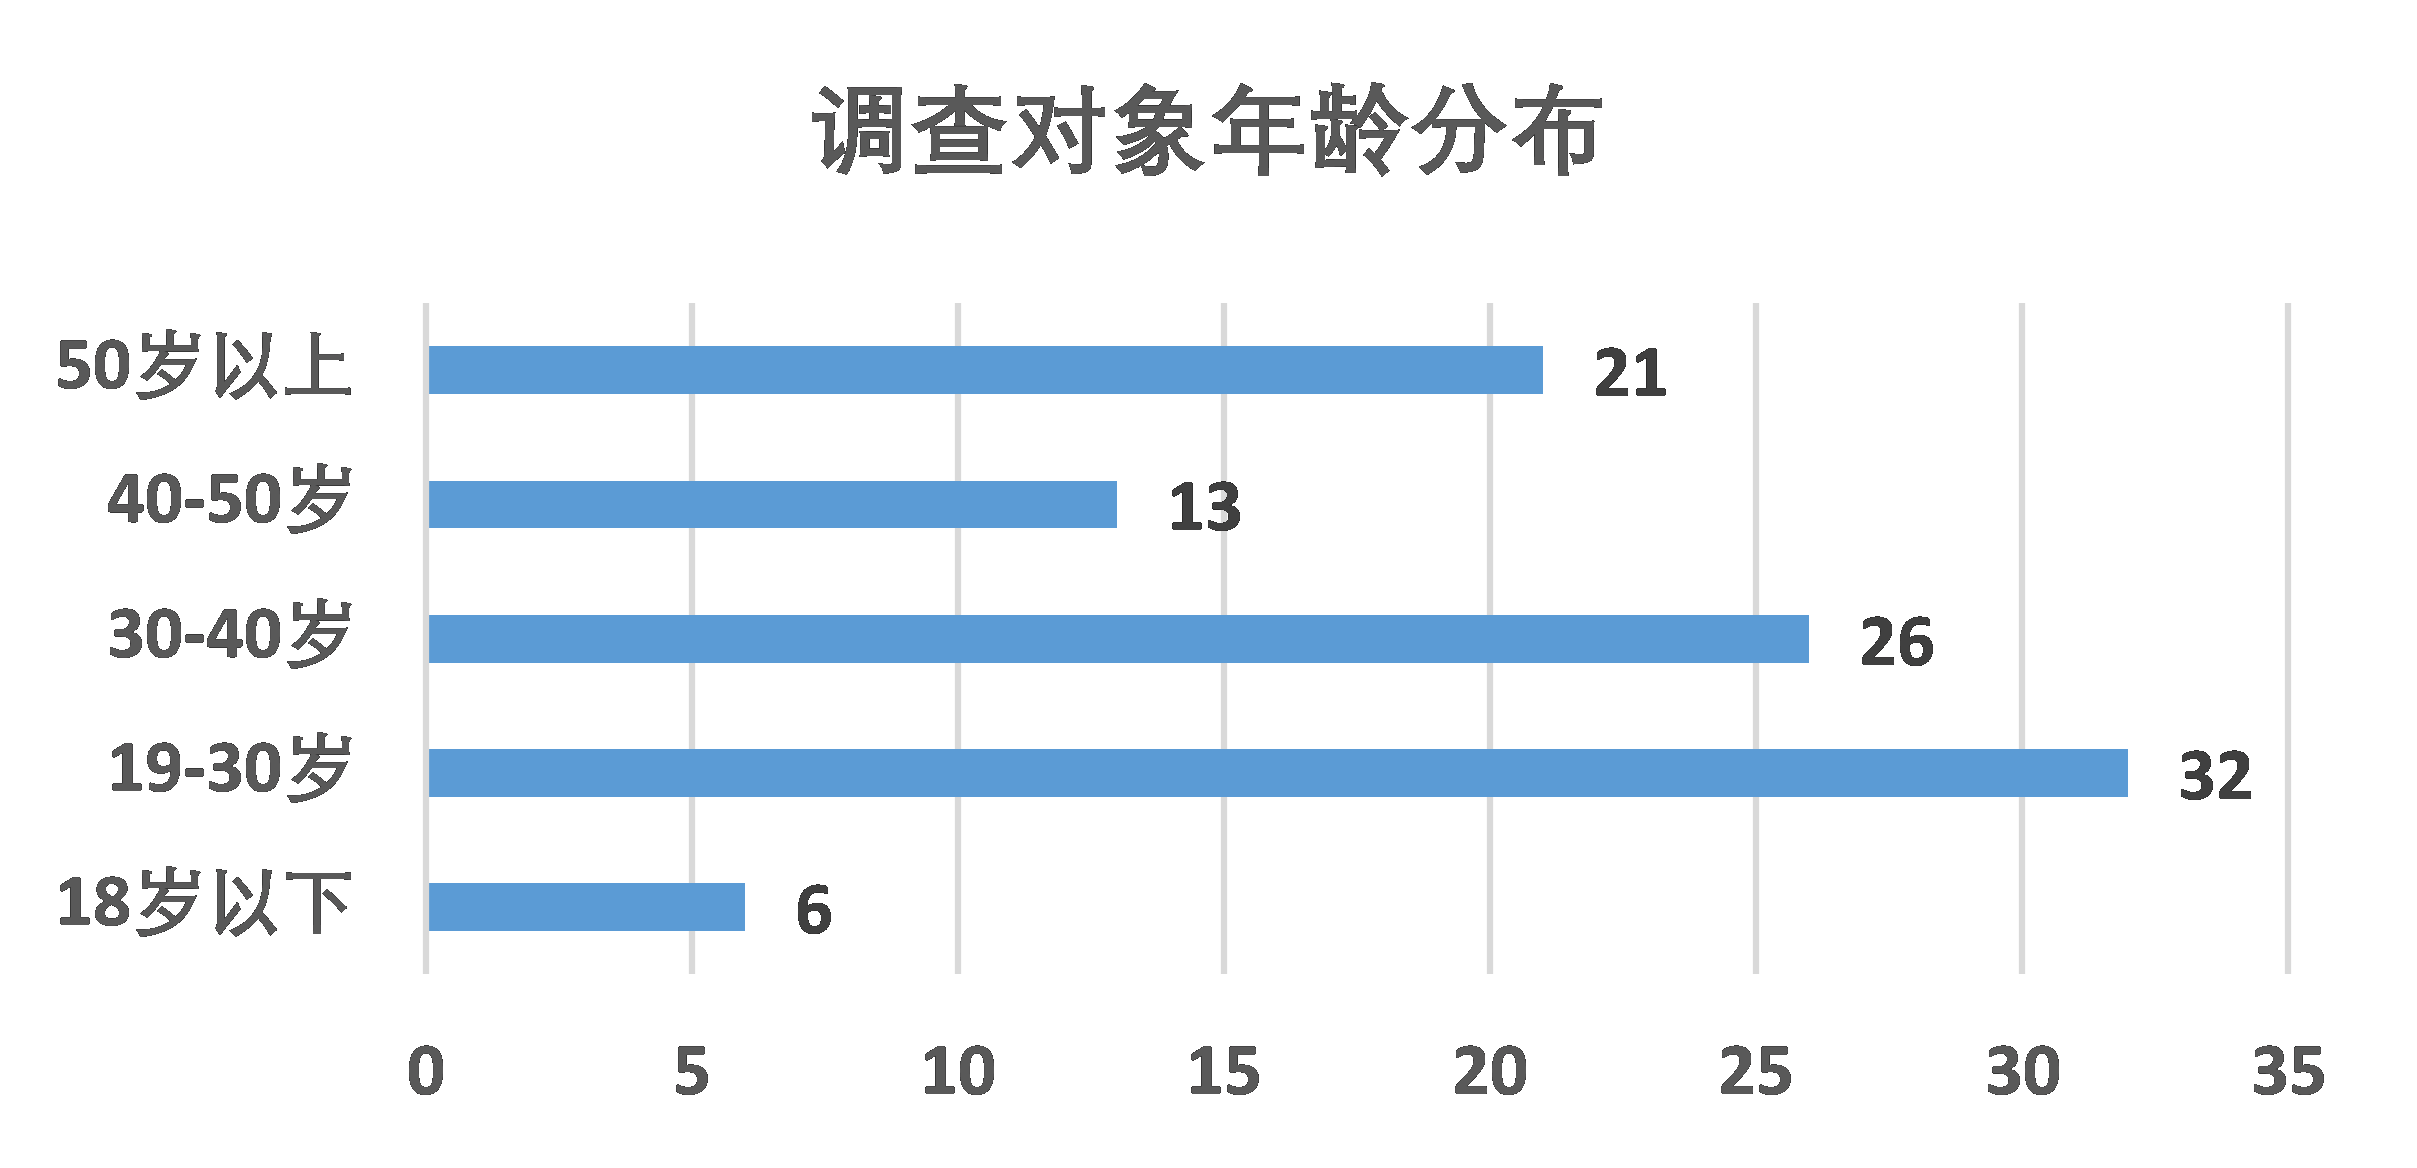
\includegraphics[height=6cm]{survey1.png}
\end{center}

\noindent \textbf{Q2.} 您平均每周网购的频率是多少?
\begin{center}
	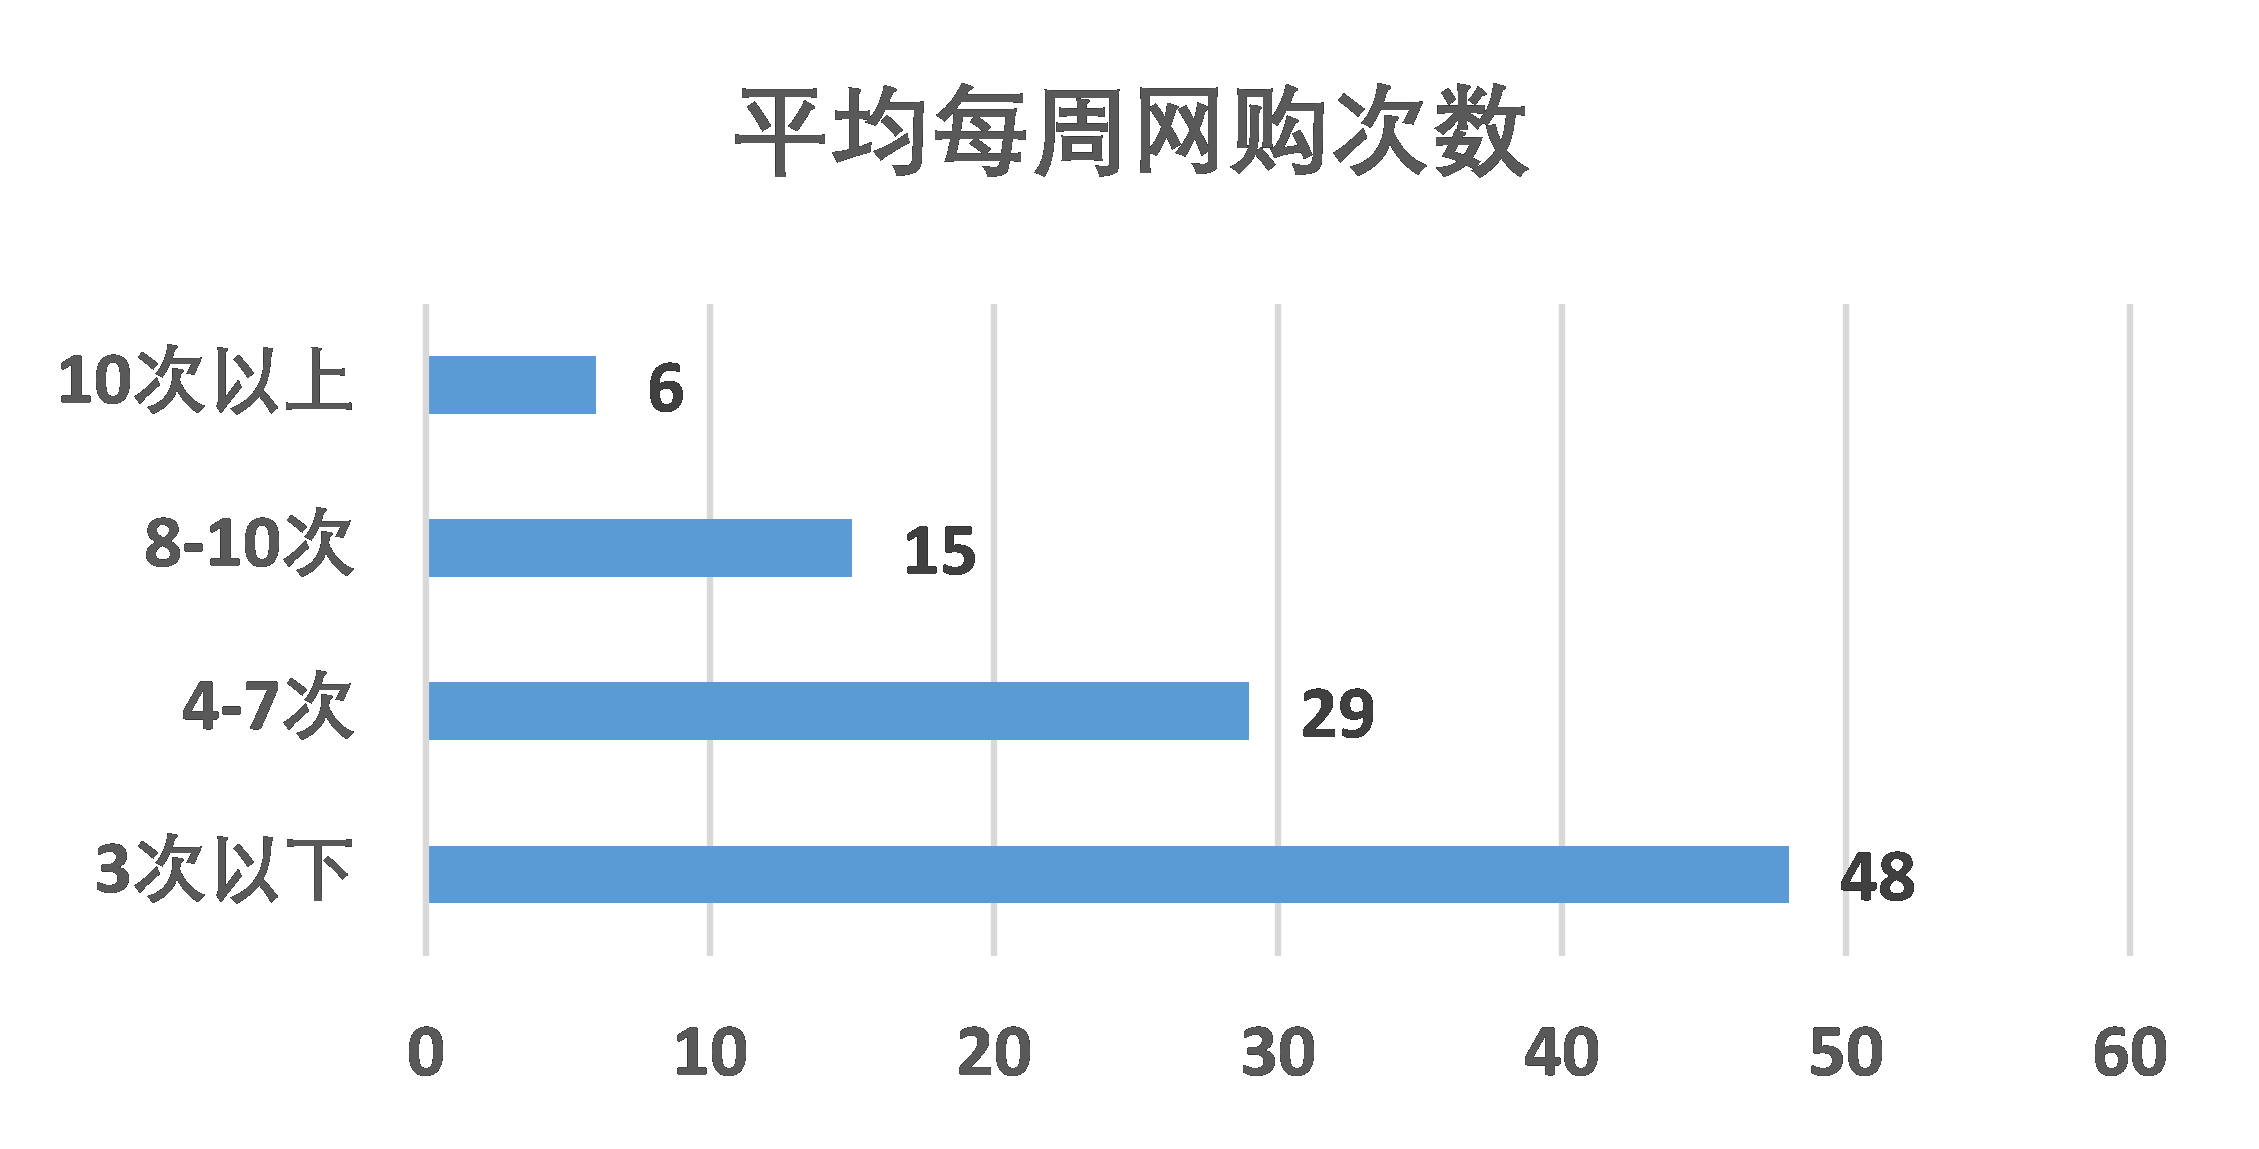
\includegraphics[height=6cm]{survey2.png}
\end{center}

\noindent \textbf{主体问题}

\noindent \textbf{Q3.} 您在网购时是否会关注物流信息?
\begin{center}
	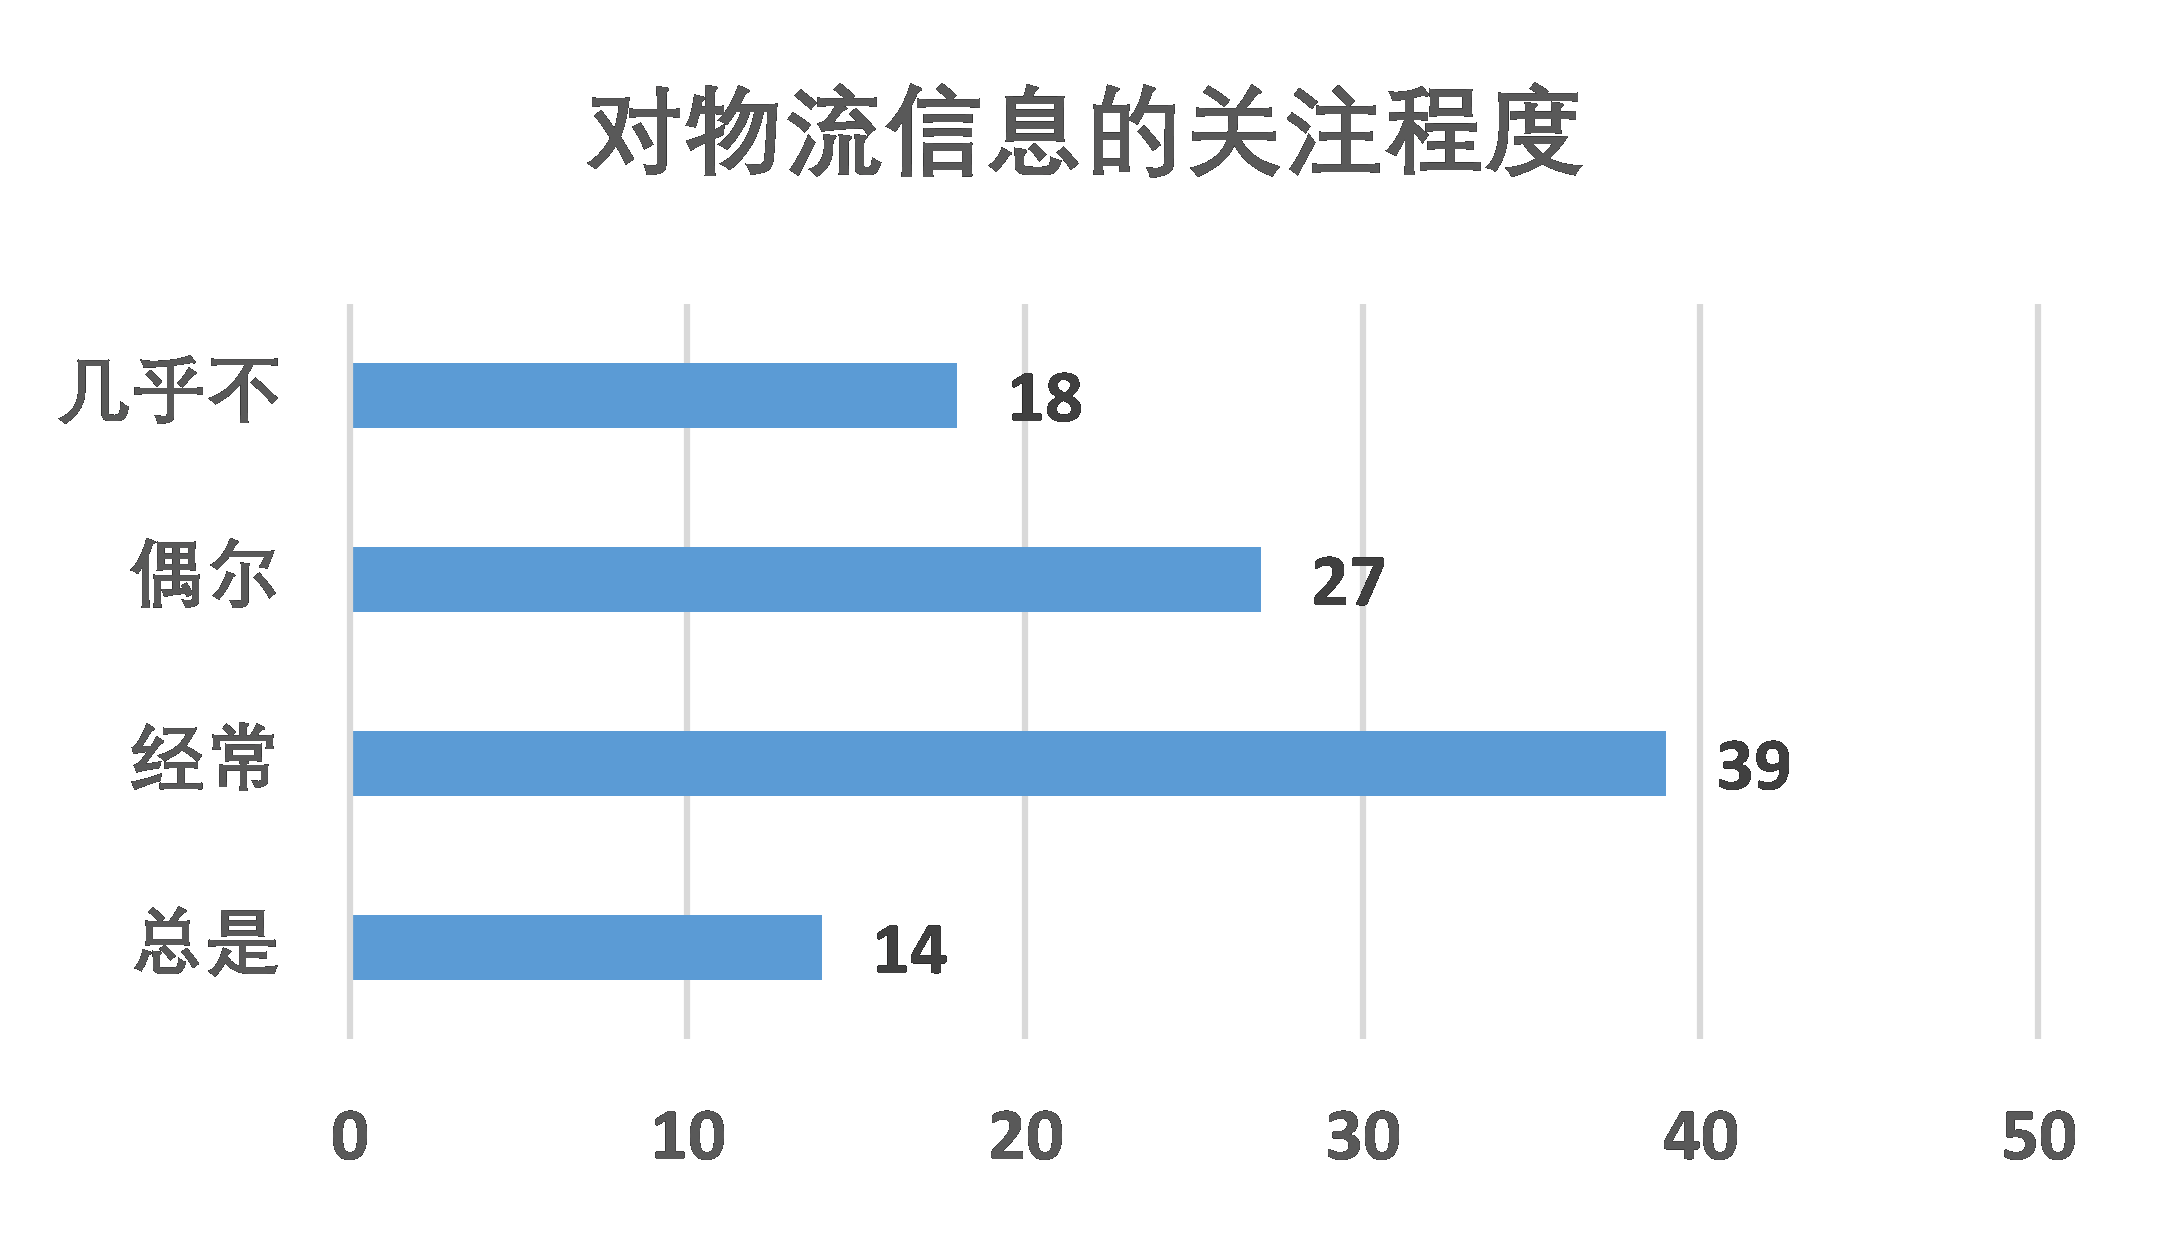
\includegraphics[height=6cm]{survey3.png}
\end{center}

\noindent \textbf{Q4.} 您对目前物流信息详细程度的呈现是否满意?
\begin{center}
	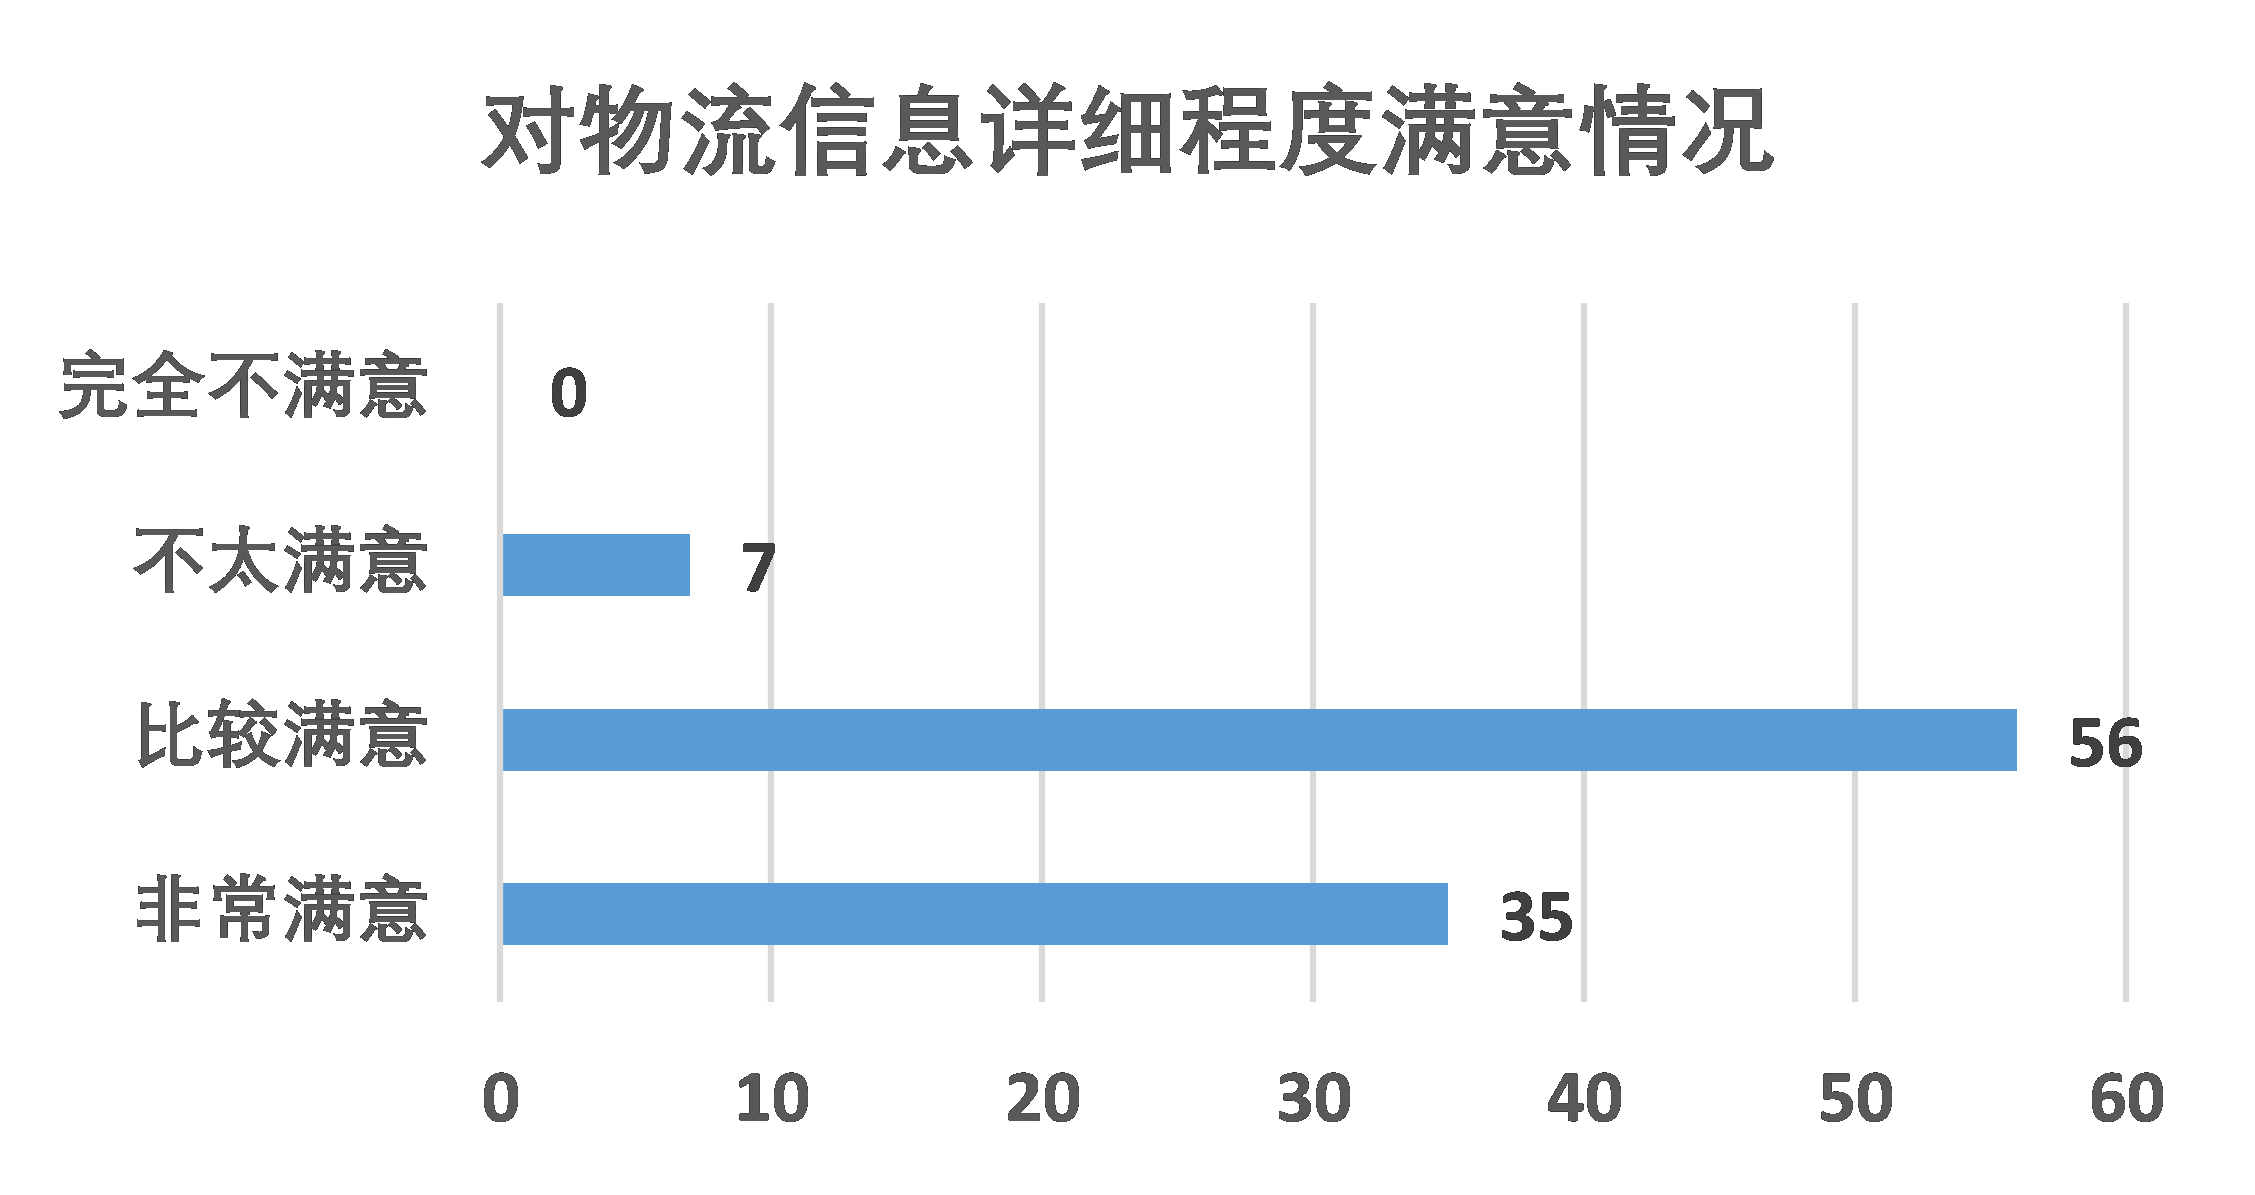
\includegraphics[height=6cm]{survey4.png}
\end{center}

\noindent \textbf{Q5.} 疫情期间,您在多大程度上相信到手的快递包裹是安全的?
\begin{center}
	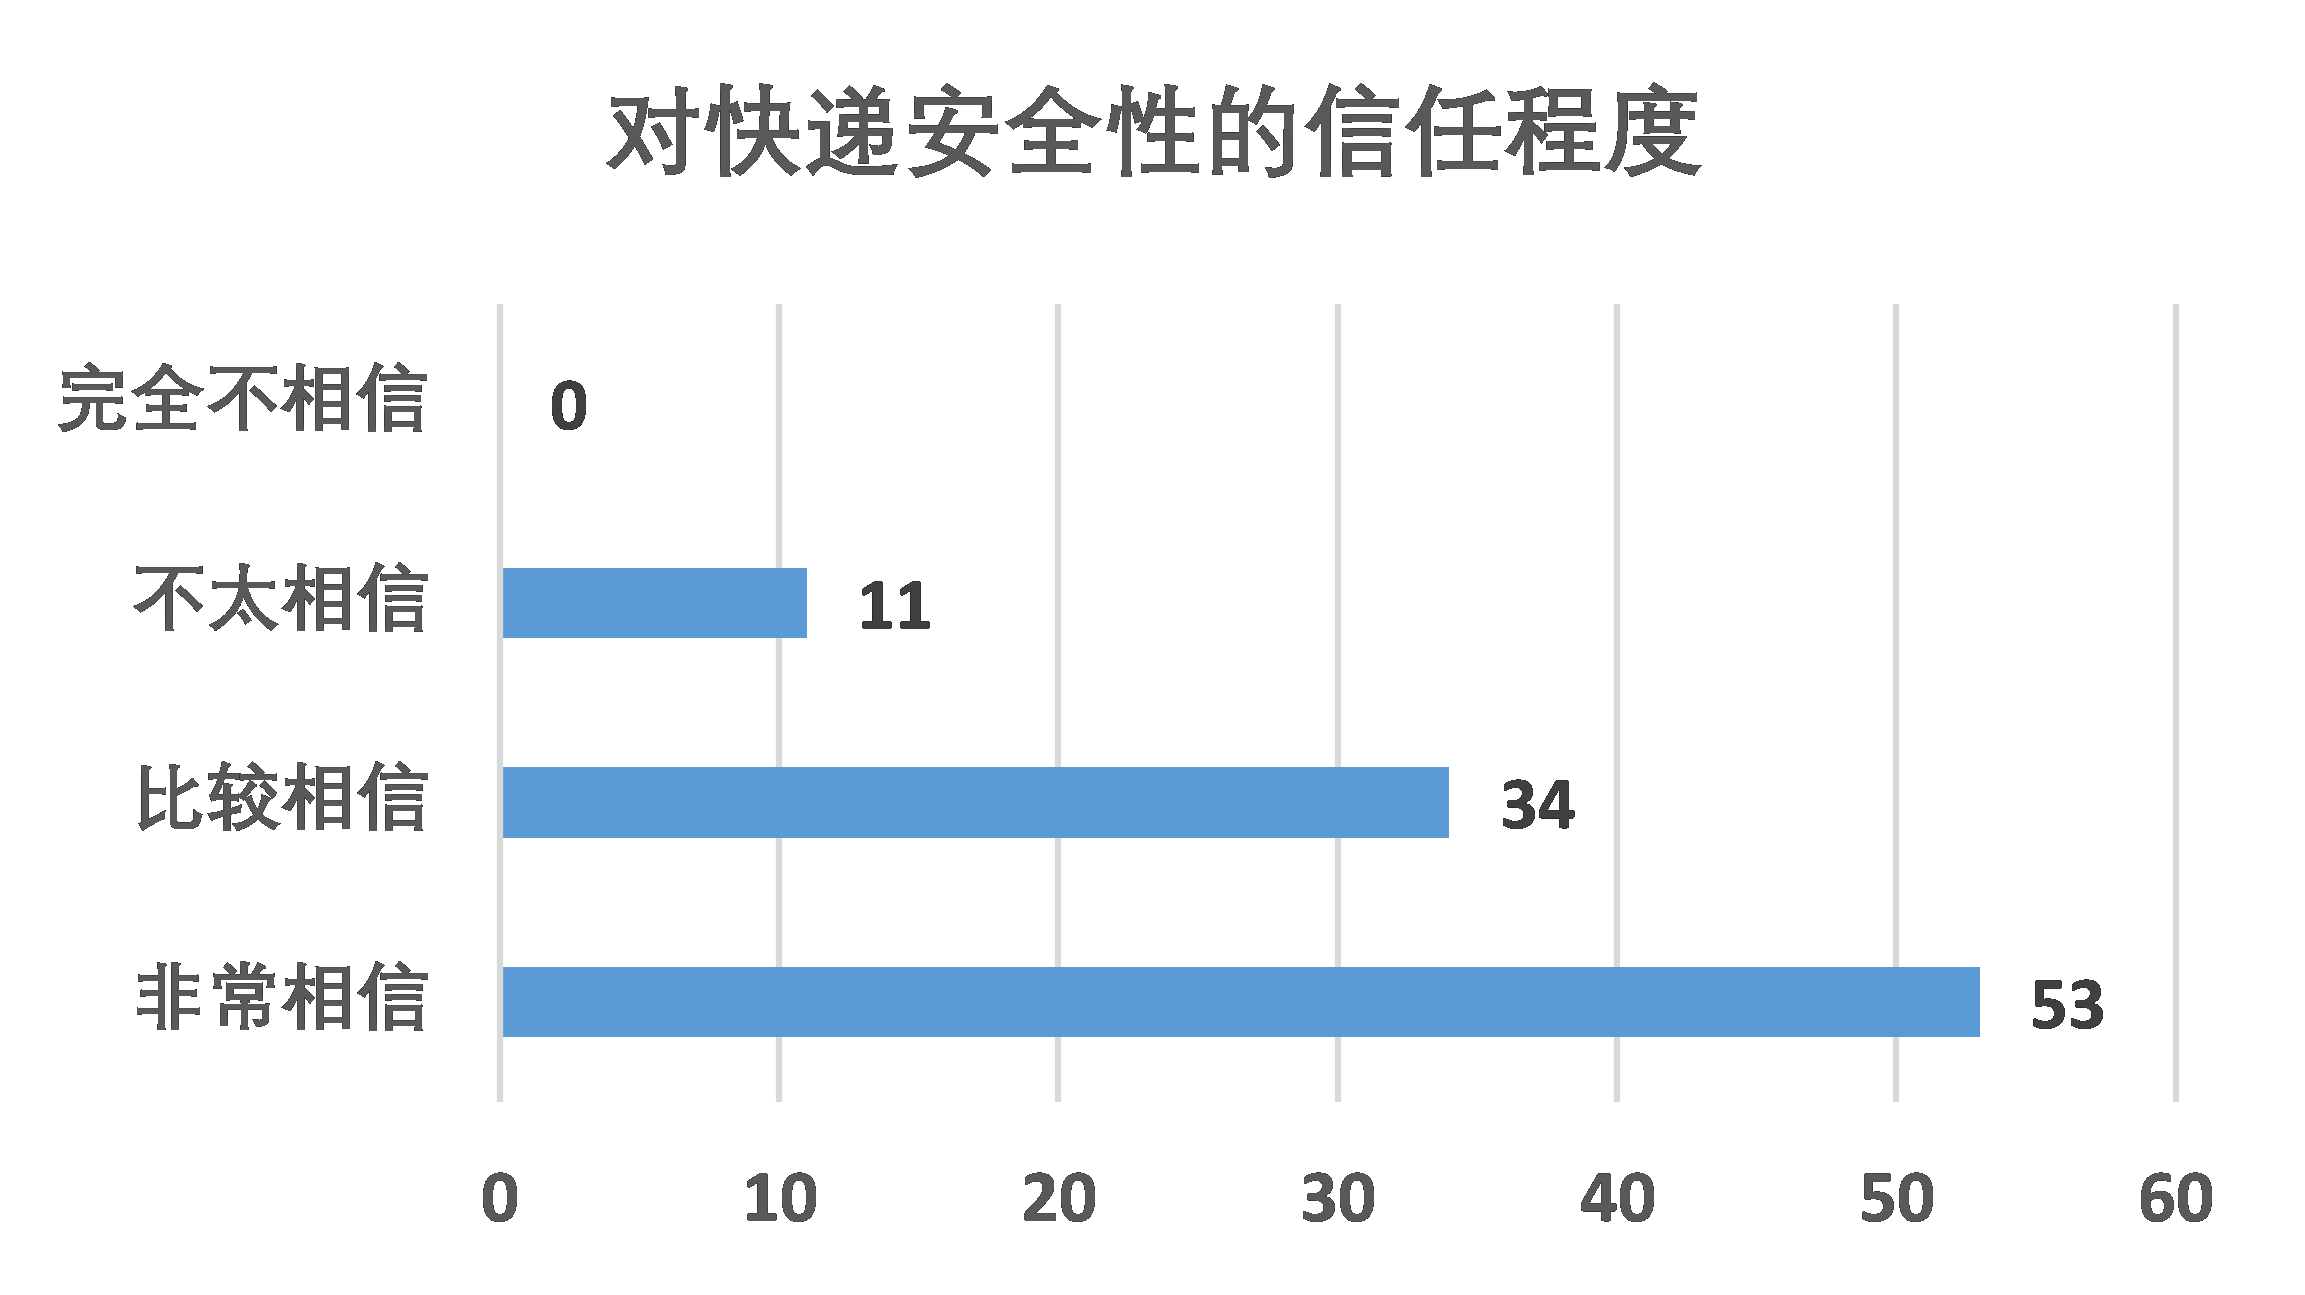
\includegraphics[height=6cm]{survey5.png}
\end{center}

\noindent \textbf{Q6.} 疫情期间,您会主动关注物流快递途径地区包含中高风险地区吗?
\begin{center}
	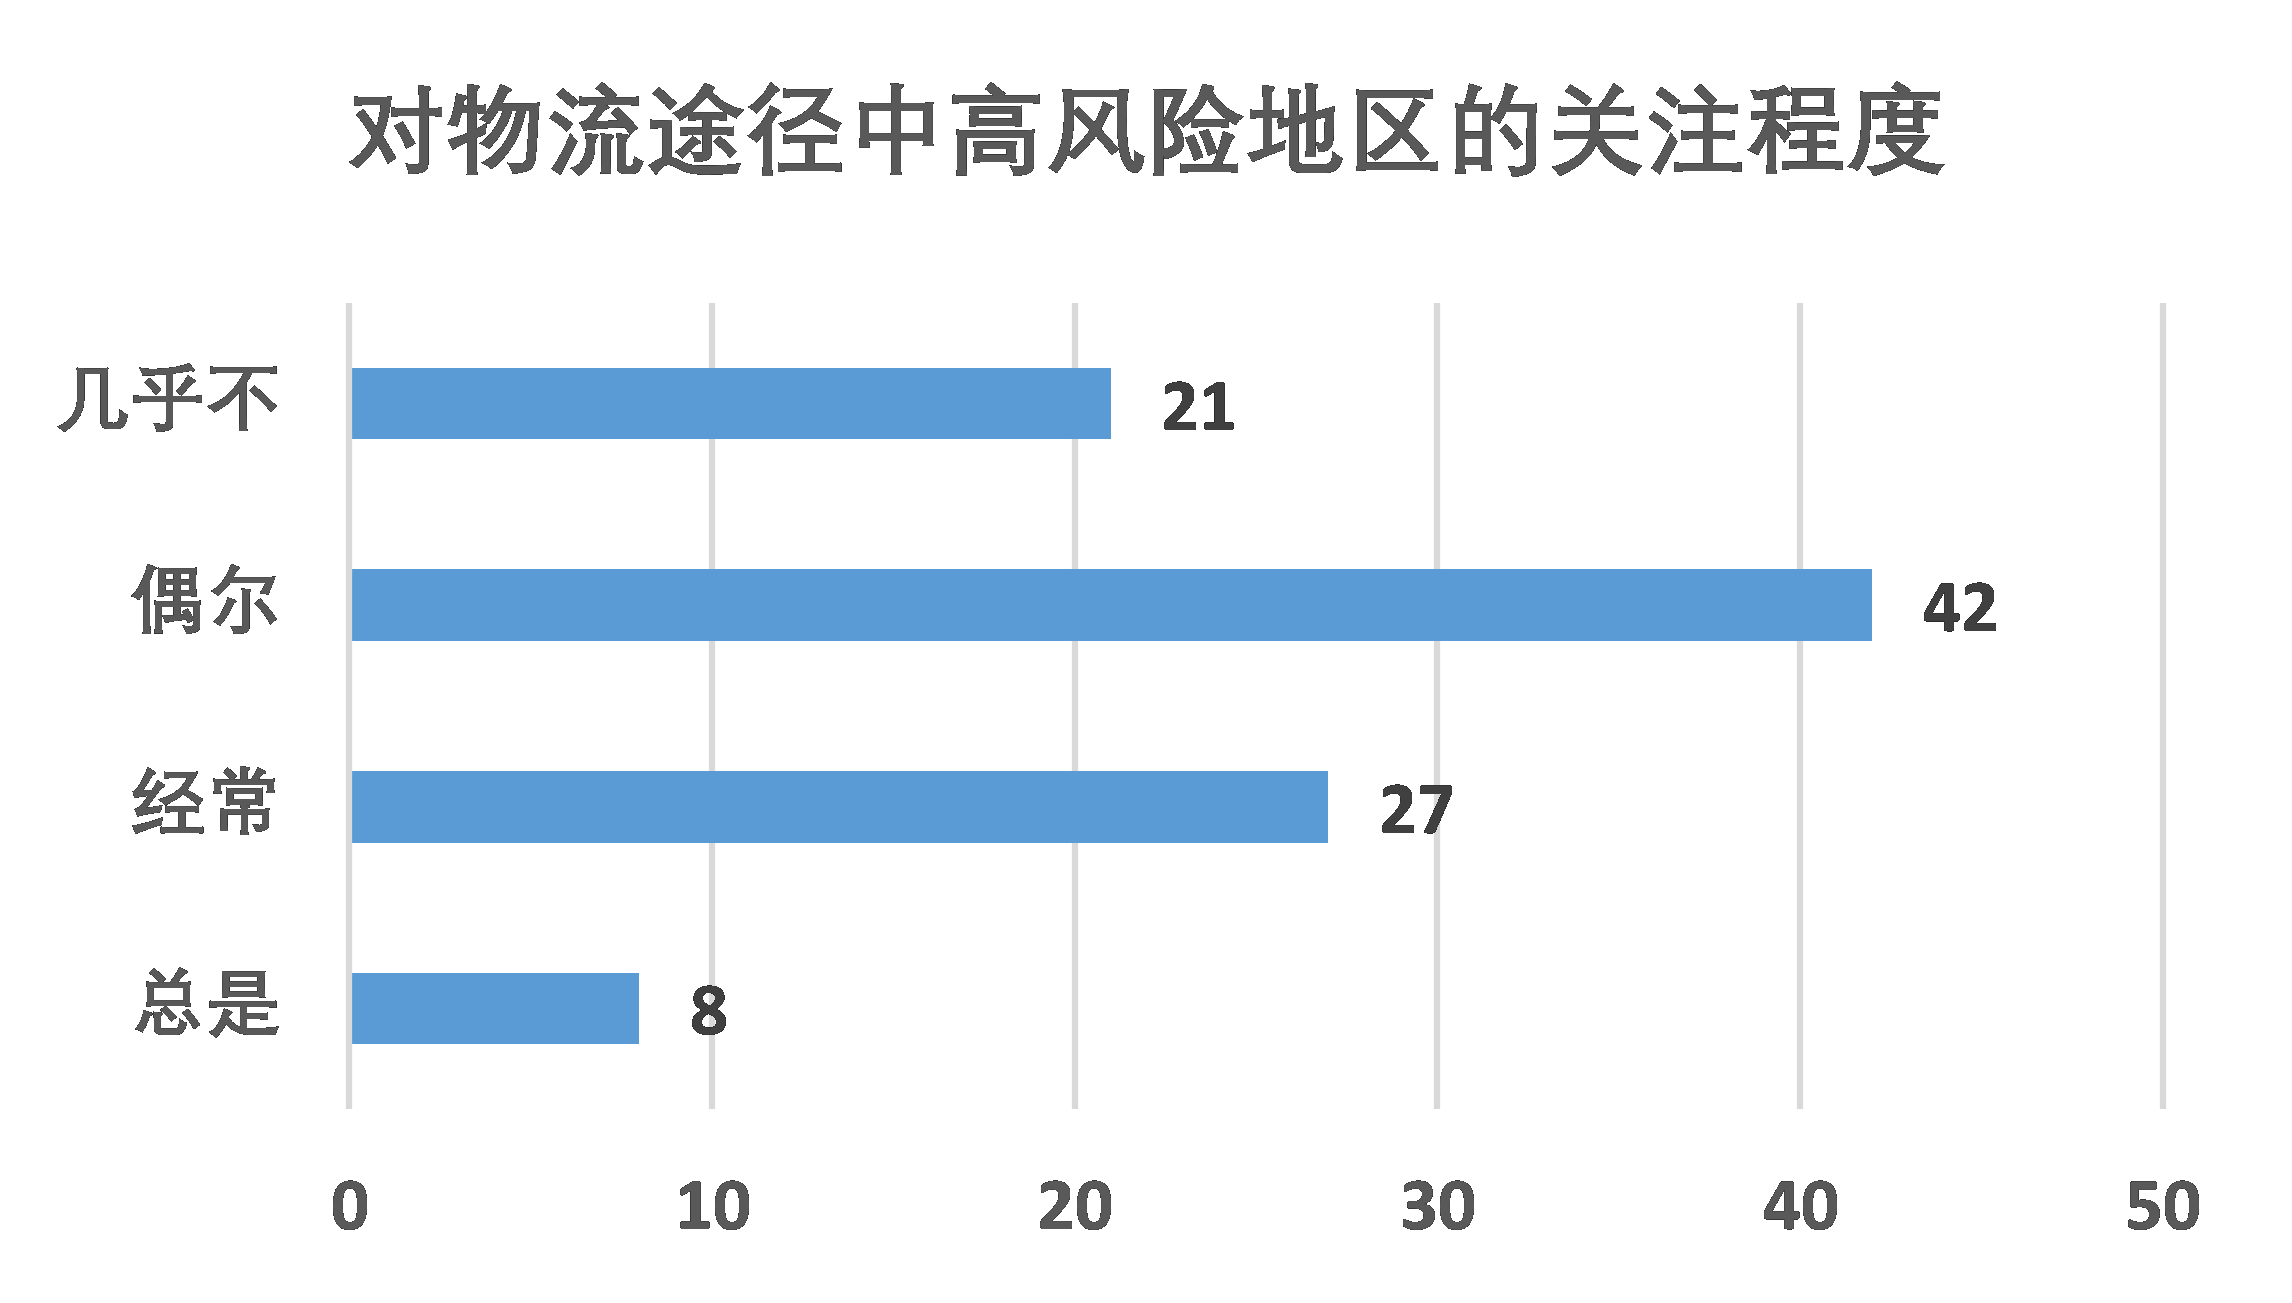
\includegraphics[height=6cm]{survey6.png}
\end{center}

\noindent \textbf{Q7.} 疫情期间,您是否会对取回的快递包裹进行消毒等防疫措施?
\begin{center}
	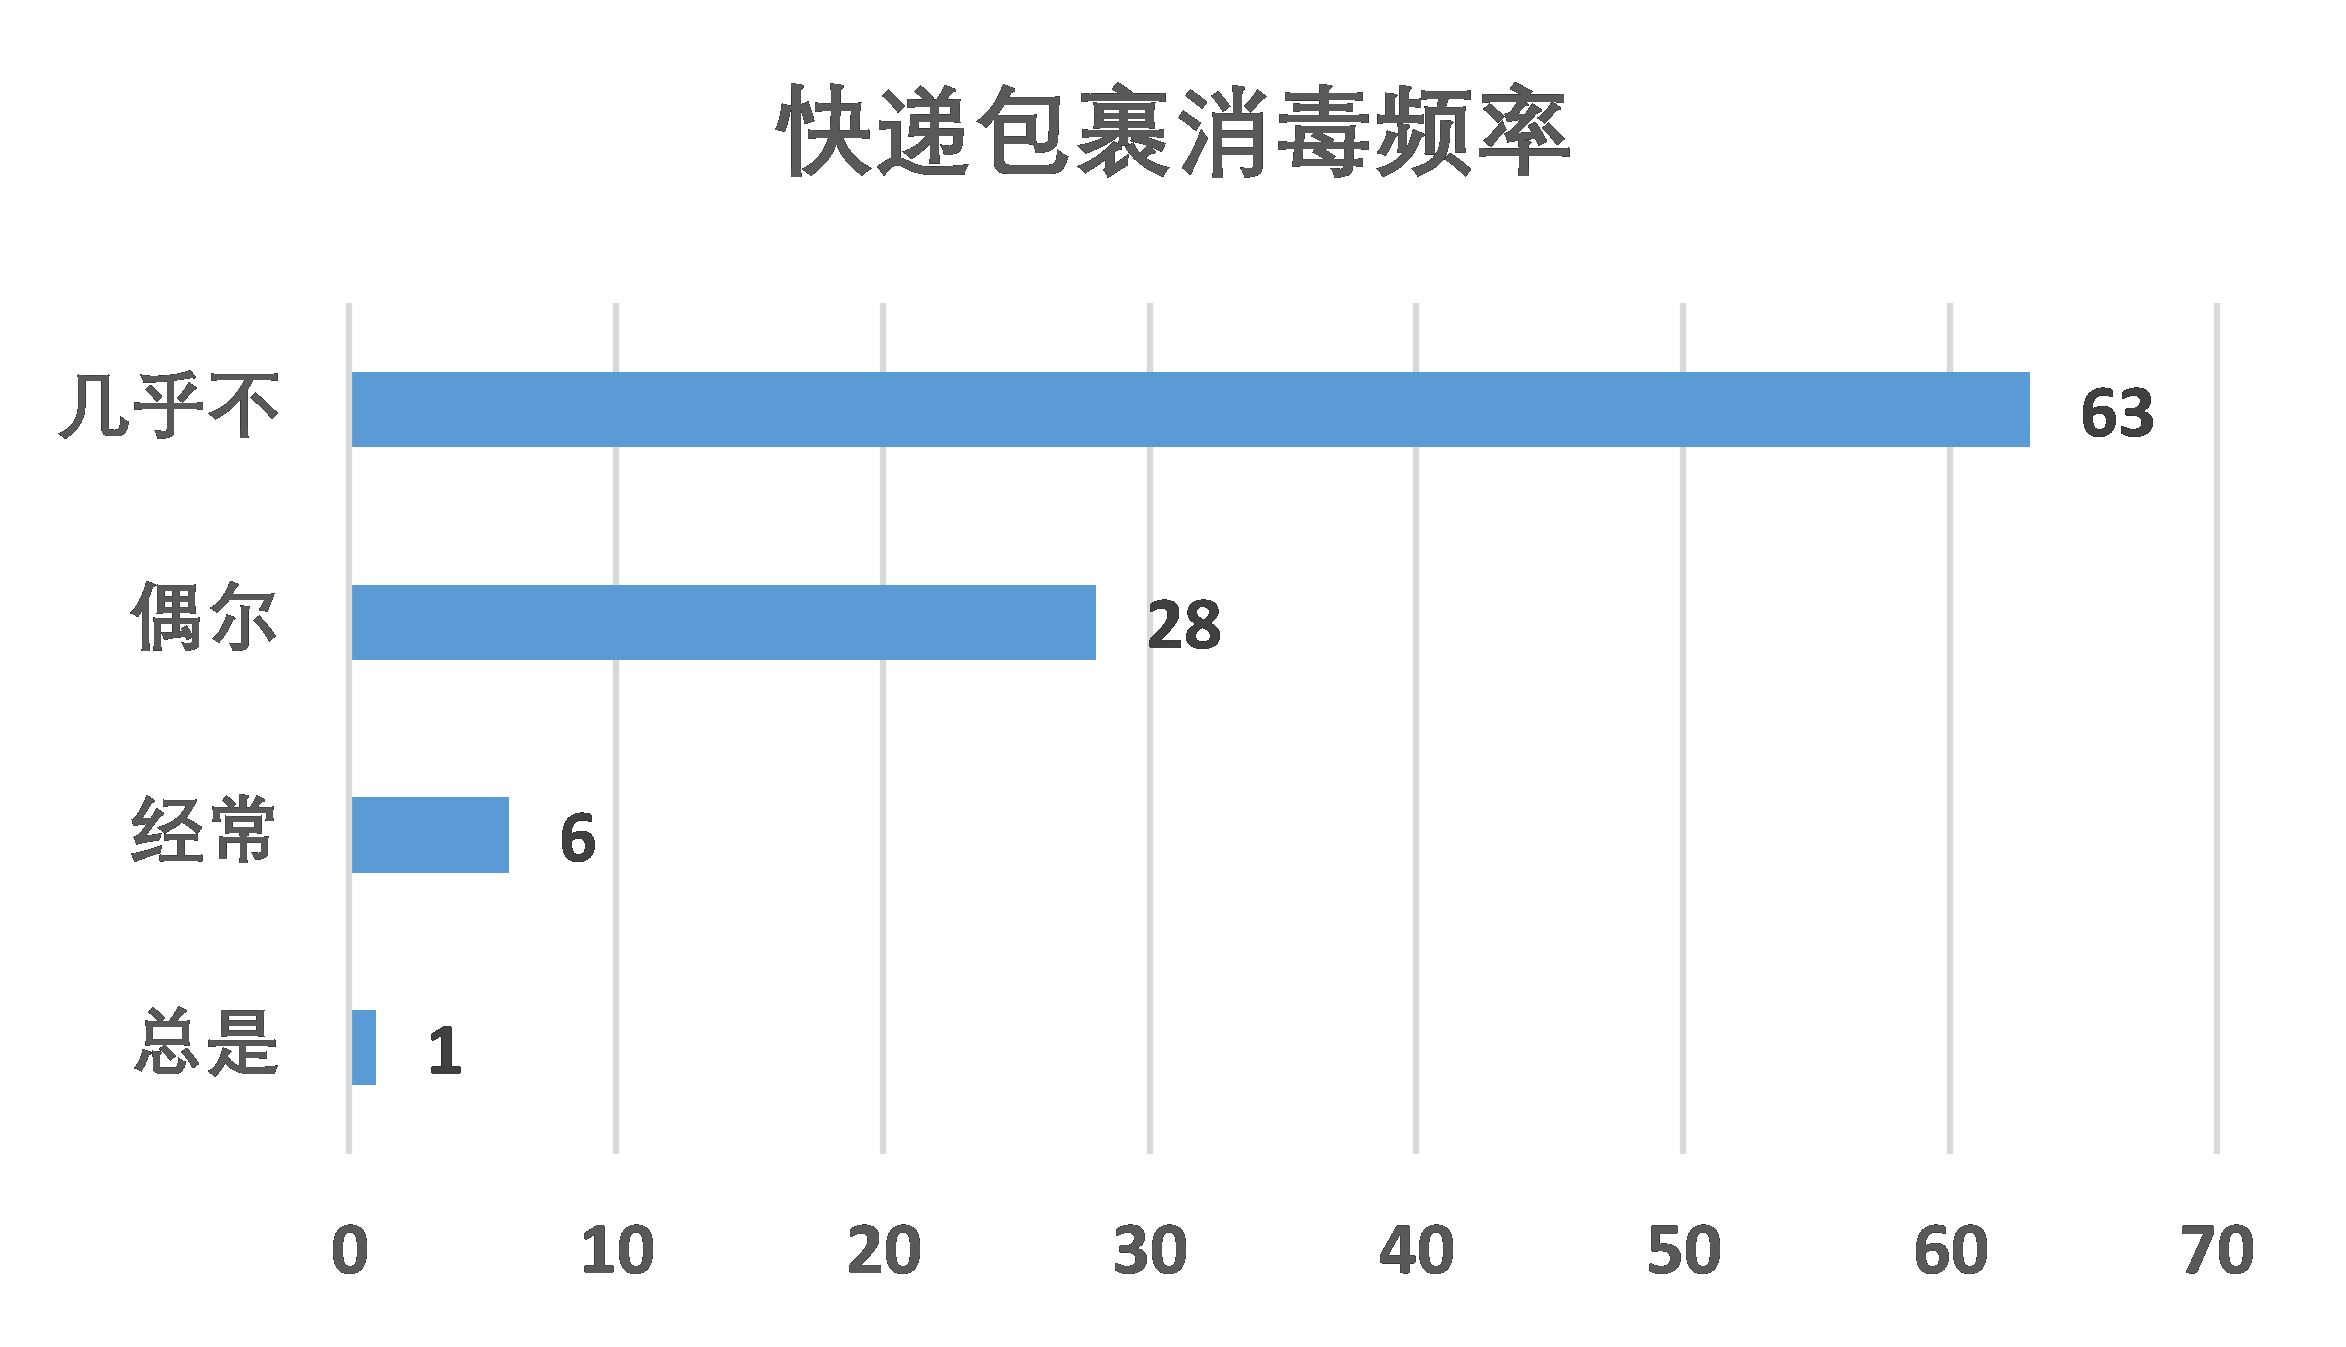
\includegraphics[height=6cm]{survey7.png}
\end{center}

\noindent \textbf{结论}

通过分析问卷结果,我们发现大约54\%的调查对象会在网购后较为经常地关注物流信息,而大约93\%的调查对象都对目前物流信息详细程度表示出满意态度。疫情防控期间,89\%的调查对象表示相信他们到手的快递是安全的,有35\%的调研对象会经常或总是关注快递途径地区是否包含中高风险地区。针对取回的快递,只有7\%的调研对象会经常或总是对包裹进行消毒措施。此外,有调研对象在问卷中表示,他们希望能够获得更直观清晰或更具警示性的提示来告诉他们可能存在的物流风险,这样他们在取快递时就会多一些防疫意识。

因此,我们希望我们建立的物流风险监测平台不仅能够更好地满足各服务对象对疫情防控期间物流管理的需求,也能通过该平台提升各方对物流风险的重视程度,从而规范自身操作,提升防疫意识,让每一份快递都能平安地送到消费者手中。

\newpage
\subsection{组织机构、用户分类及业务流程}

\subsubsection{组织机构}

\noindent \textbf{电商平台组织机构}
\begin{center}
	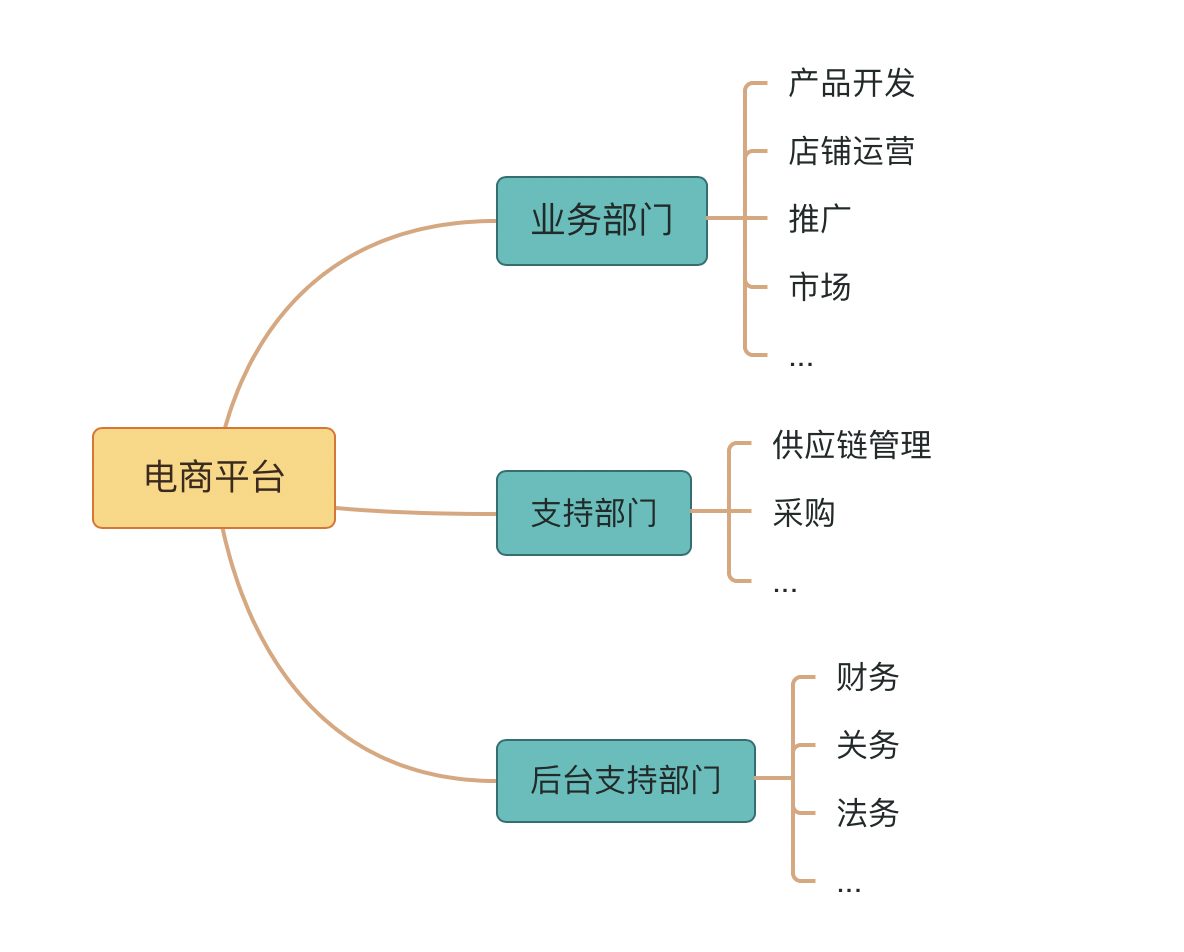
\includegraphics[height=8cm]{e-cormmerce_organization.png}
\end{center}

\noindent \textbf{物流公司组织机构}
\begin{center}
	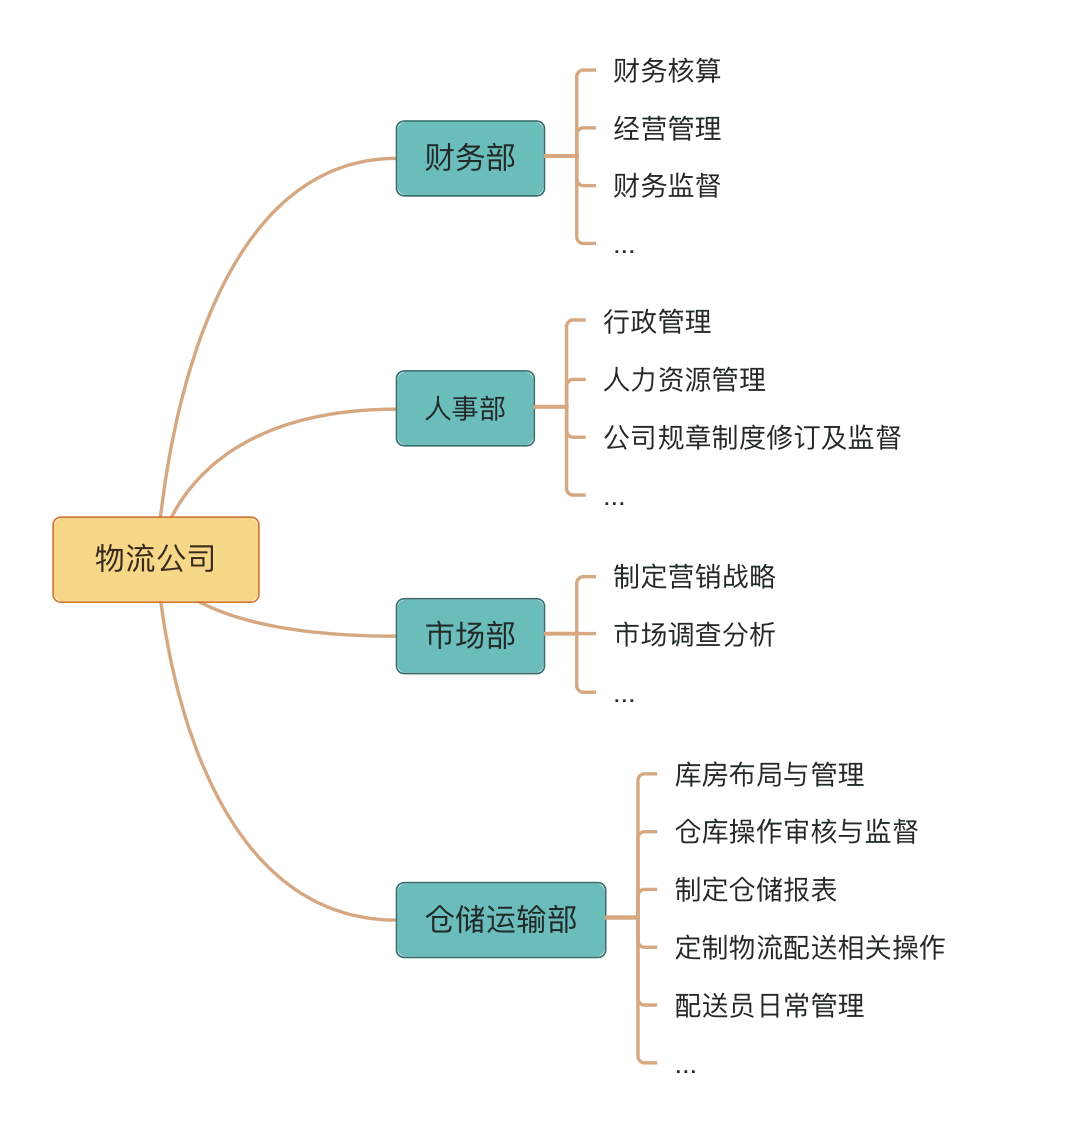
\includegraphics[height=12cm]{logistics_organization.png}
\end{center}

\subsubsection{用户分类}

\noindent \textbf{物流公司}
\begin{itemize}
	\item 输入:物流管理、配送人员每日健康状况以及配送信息。
	\item 输入:运输包裹信息以及包裹配送所经地。
	\item 查询:特定包裹的配送状态与配送人员、产品相关信息。
	\item 查看特定时间段内包裹相关信息分析报告。
	\item 查看特定时间段内物流成本收益分析报告。
	\item 实现疫情下物流配送人员及包裹管理:对标国家卫生健康委员会官方网站,即使标注途径标为中高风险地区的人员及包裹。
\end{itemize}

\noindent \textbf{电商平台}
\begin{itemize}
	\item 输入:订单信息(包括买家、卖家信息)。
	\item 查询:卖家基本信息及相关售卖商品信息及配送状况。
	\item 查询:买家基本信息及相关购买商品信息及配送状况。
	\item 查询:特定包裹的配送状态与配送人员、产品相关信息。
	\item 查看电商平台成本收益分析报告。
	\item 查看特定时间段内电商平台总体订单配送信息分析报告。
\end{itemize}

\noindent \textbf{卖家}
\begin{itemize}
	\item 输入:卖家基本信息及对应相关电商平台的特定序列号。
	\item 查询:相关售卖商品信息及配送状况。
\end{itemize}

\noindent \textbf{买家}
\begin{itemize}
	\item 输入:买家基本信息。
	\item 查询:相关购买商品信息及配送状况。
\end{itemize}

\noindent \textbf{游客(进入网站未登录)}
\begin{itemize}
	\item 查看平台主业务。
	\item 对标国家卫生健康委员会官方网站,查看中高风险地区总地图及相关信息。
\end{itemize}

\subsubsection{业务流程}

\noindent \textbf{(1) 物流订单数据管理服务}
\begin{center}
	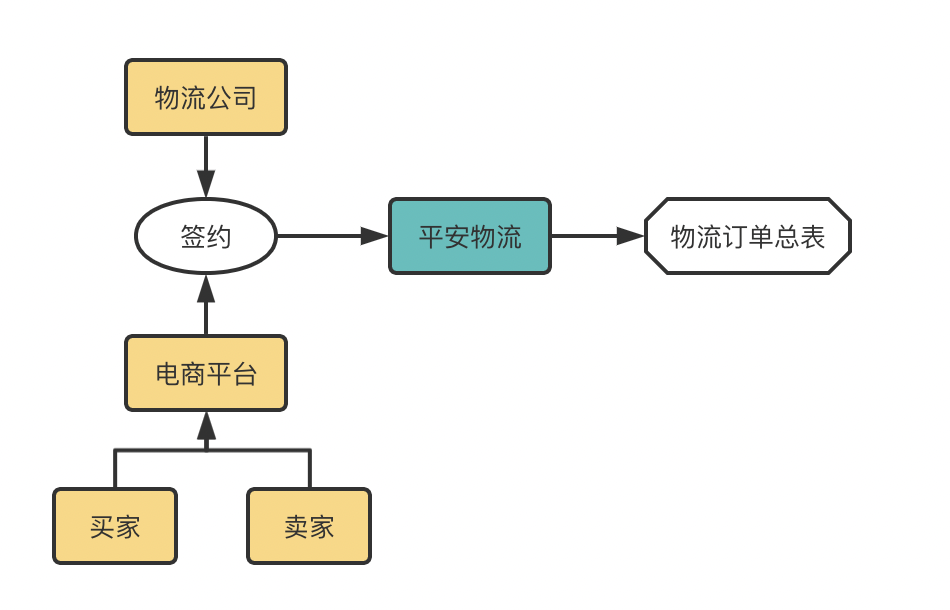
\includegraphics[height = 8cm]{logistics_order_mag.png}
\end{center}

\noindent \textbf{(2) 查询特定信息服务}
\begin{center}
	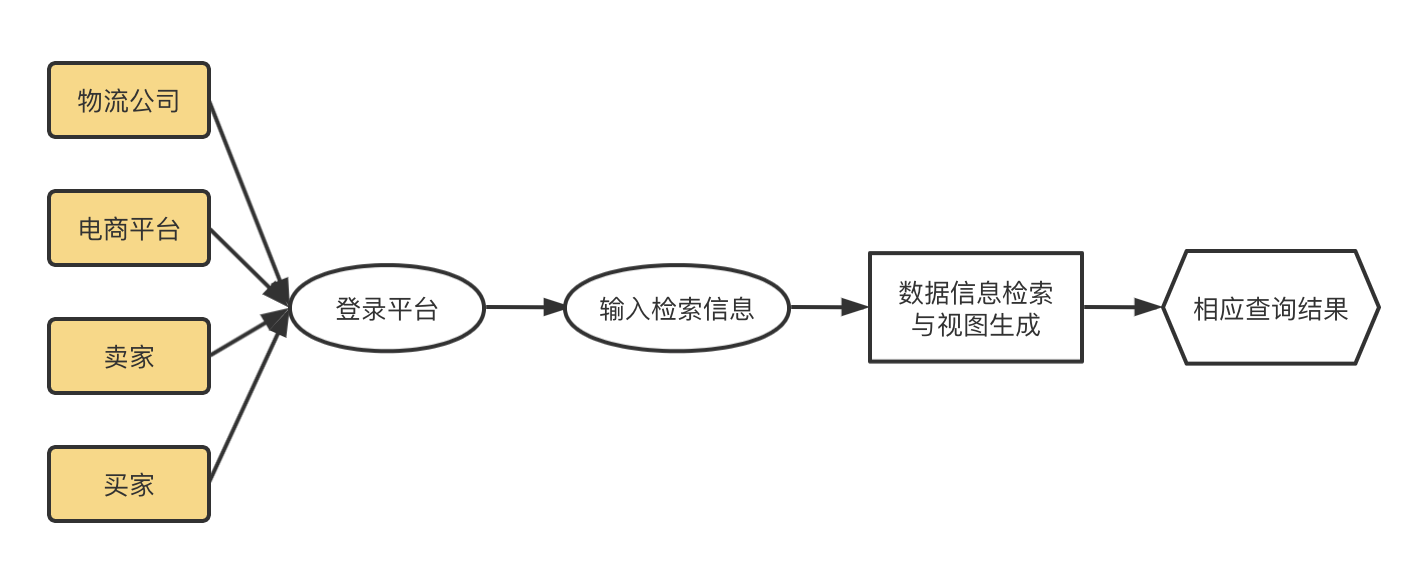
\includegraphics[height = 6cm]{query_info.png}
\end{center}

\noindent \textbf{(3) 查看特定分析报告服务}
\begin{center}
	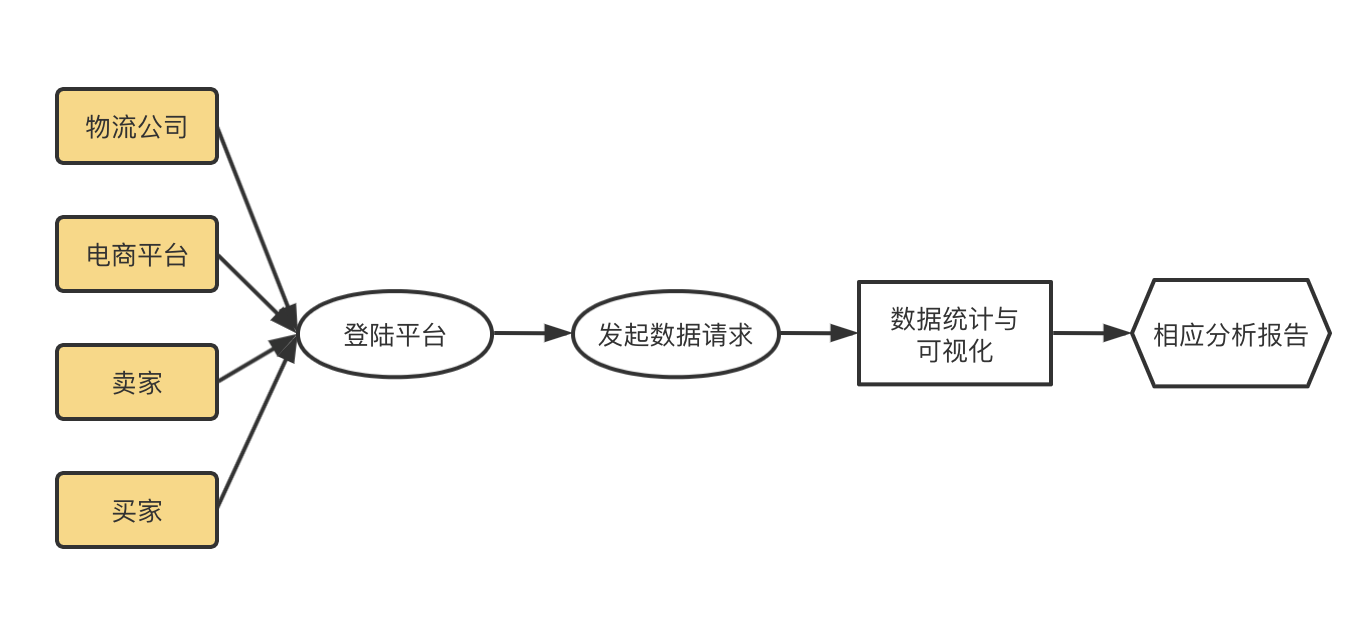
\includegraphics[height = 6cm]{query_report.png}
\end{center}

\noindent \textbf{(4) 查看中高风险地区地图及相关信息服务}
\begin{center}
	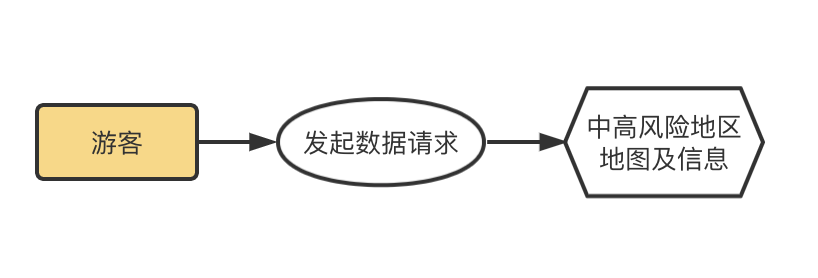
\includegraphics[height = 4cm]{cov_map.png}
\end{center}

\noindent \textbf{(5) 数据统计与可视化流程}
\begin{center}
	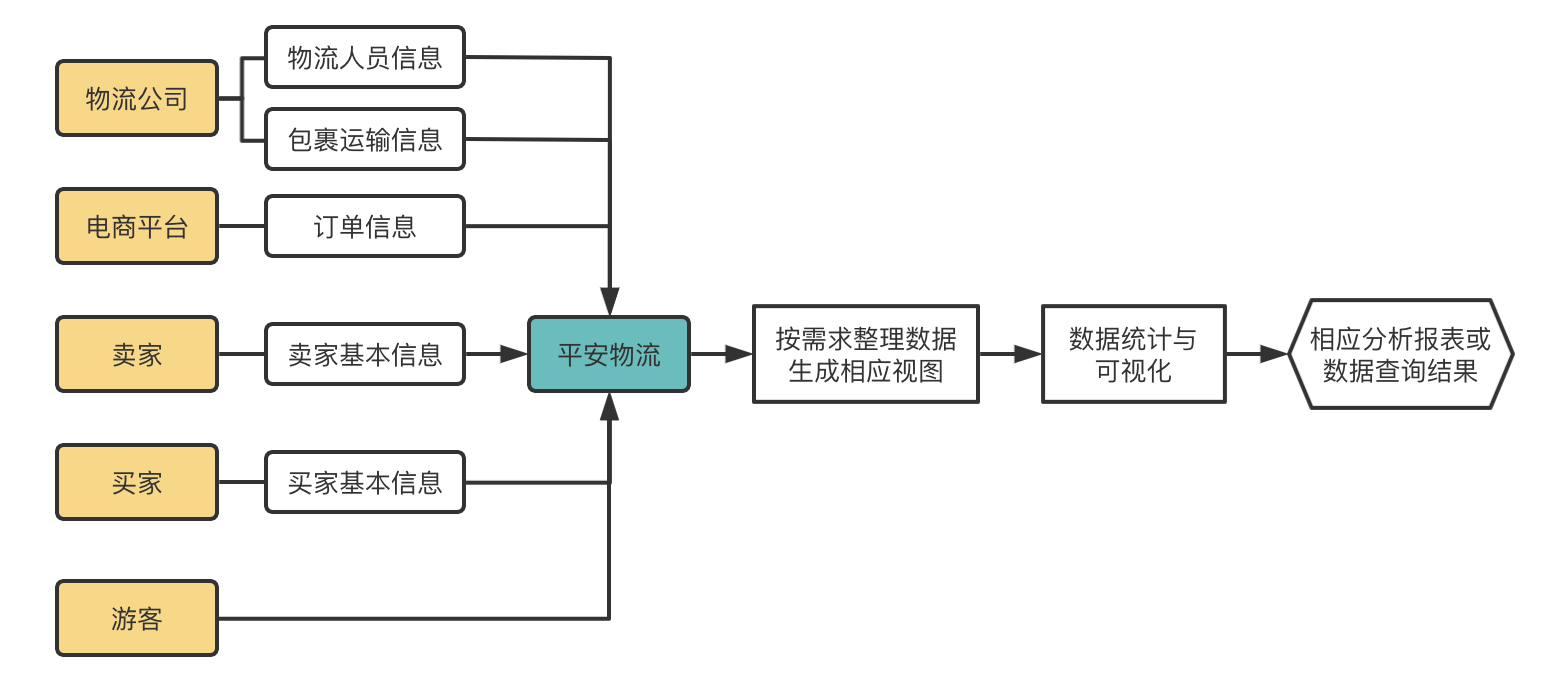
\includegraphics[height = 6.7cm]{data_visualization.png}
\end{center}

\newpage
\subsection{数据流图}

\subsubsection{第一层数据流图}

\begin{center}
	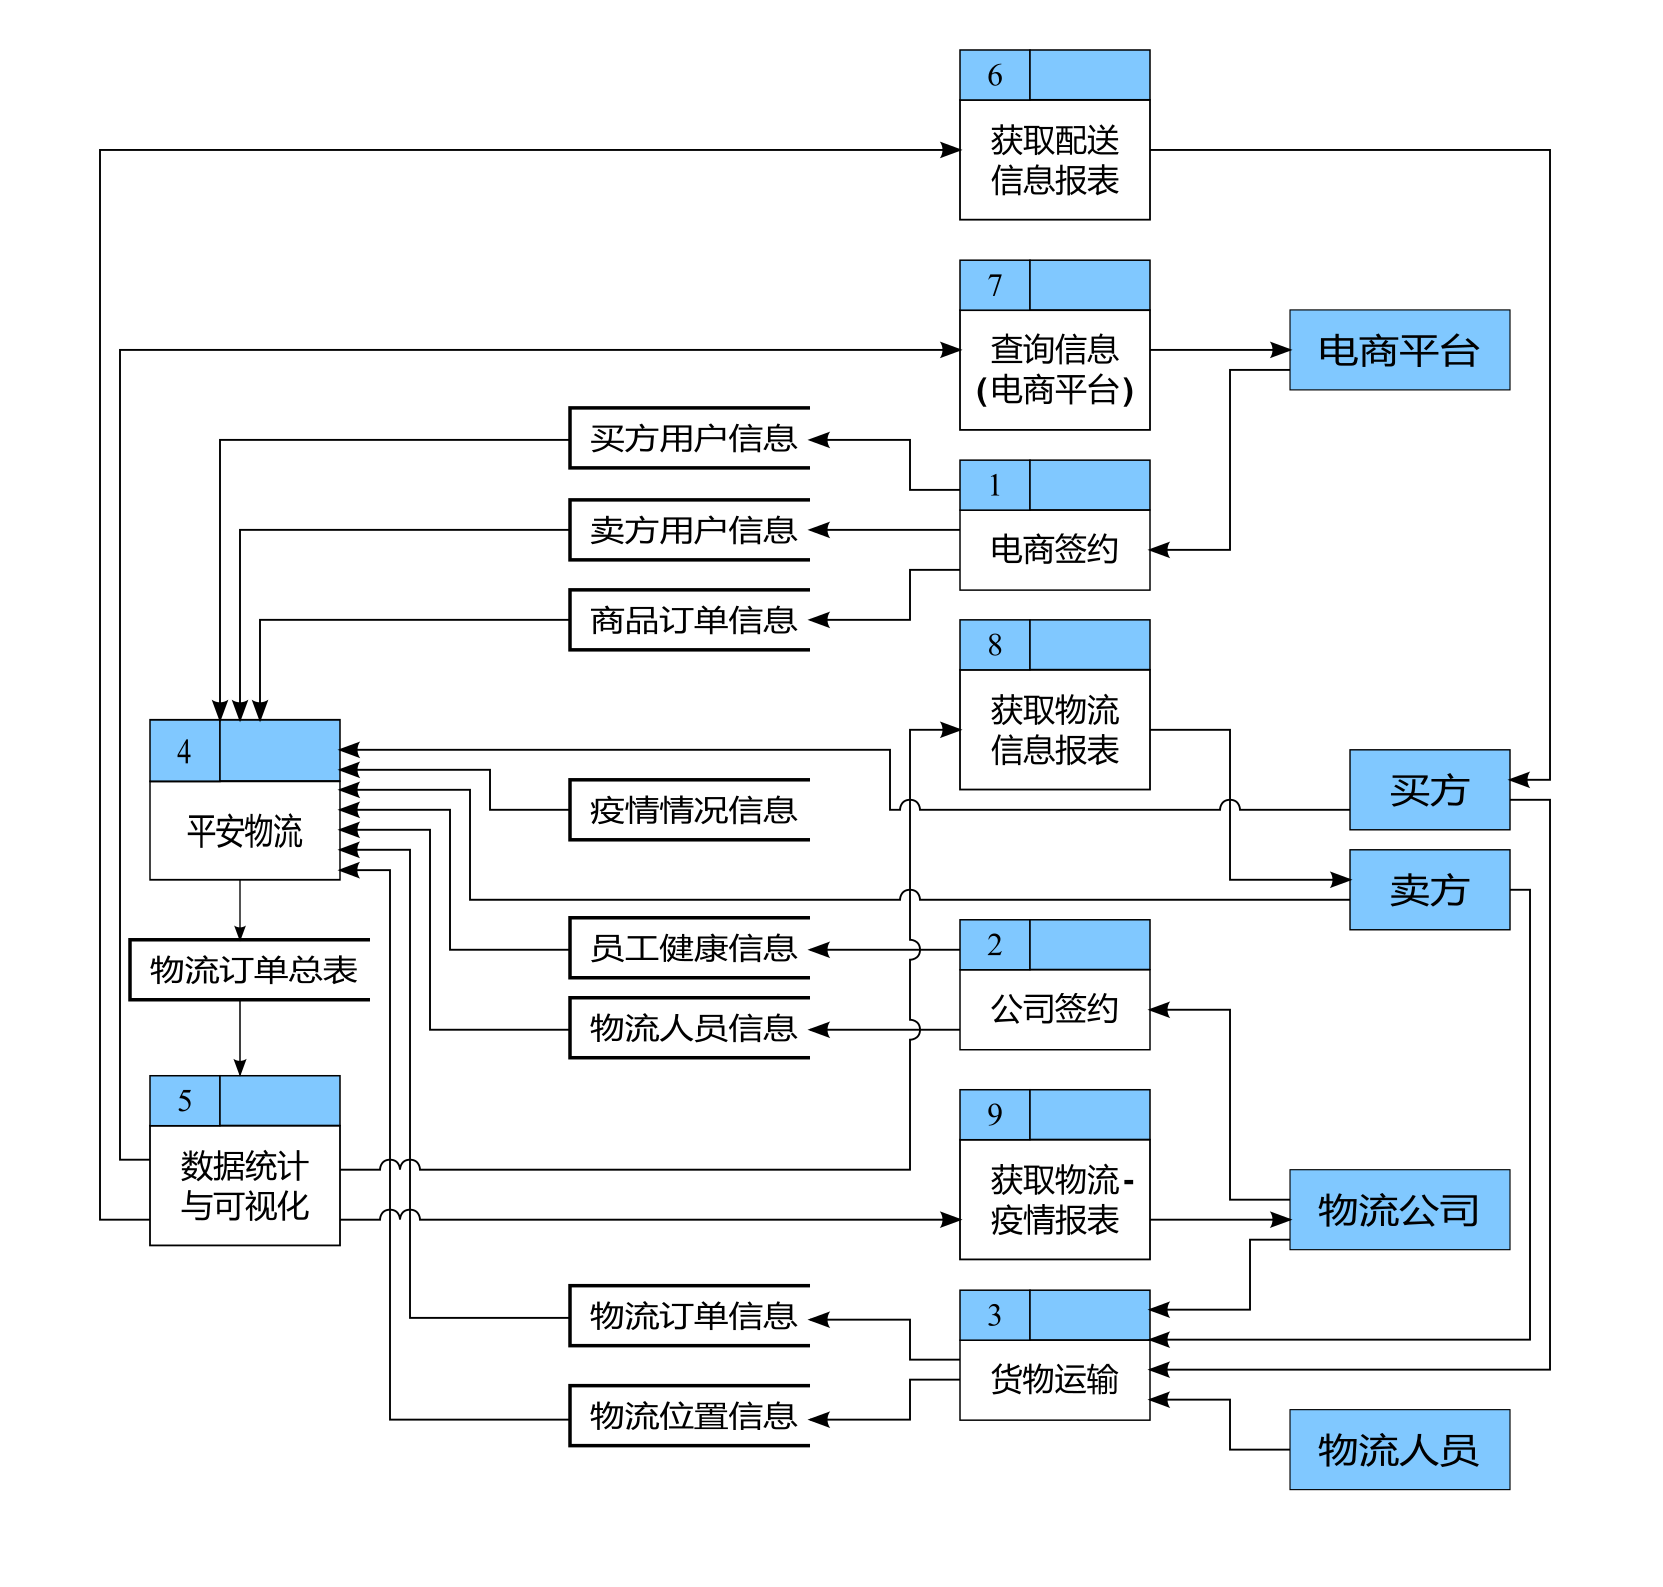
\includegraphics[height = 20cm]{level-1.png}
\end{center}

\subsubsection{第二层数据流图}

\noindent \textbf{(1) 提交物流订单}
\begin{center}
	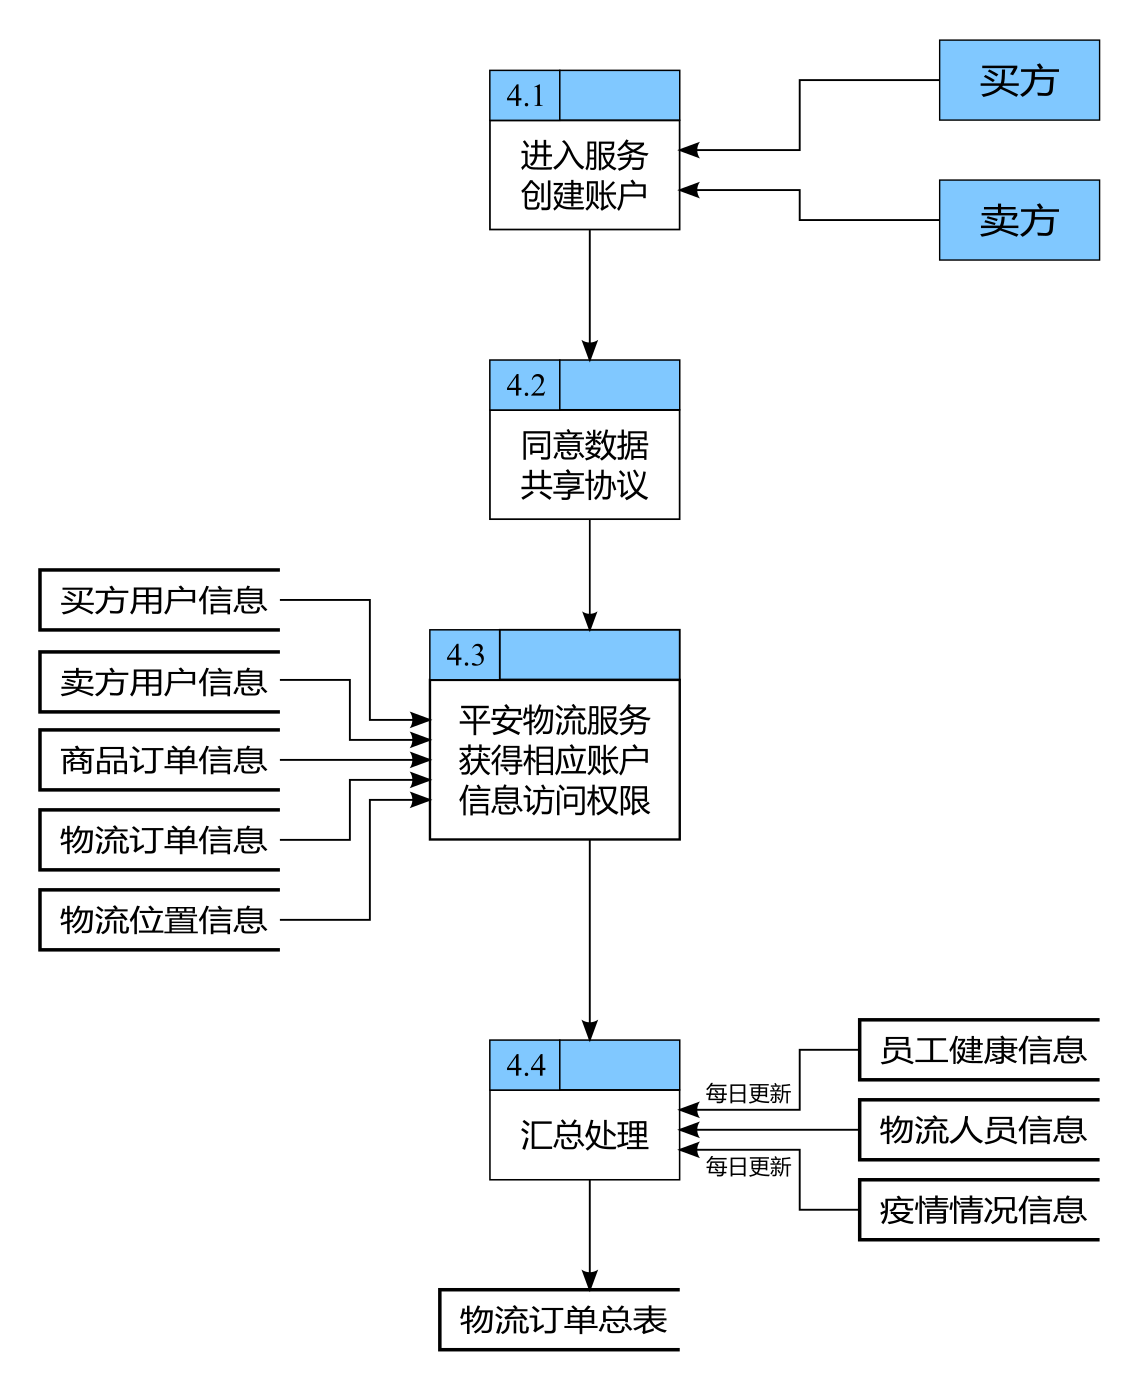
\includegraphics[height = 8cm]{level-2.1.png}
\end{center}

\noindent \textbf{(2) 安排配送}
\begin{center}
	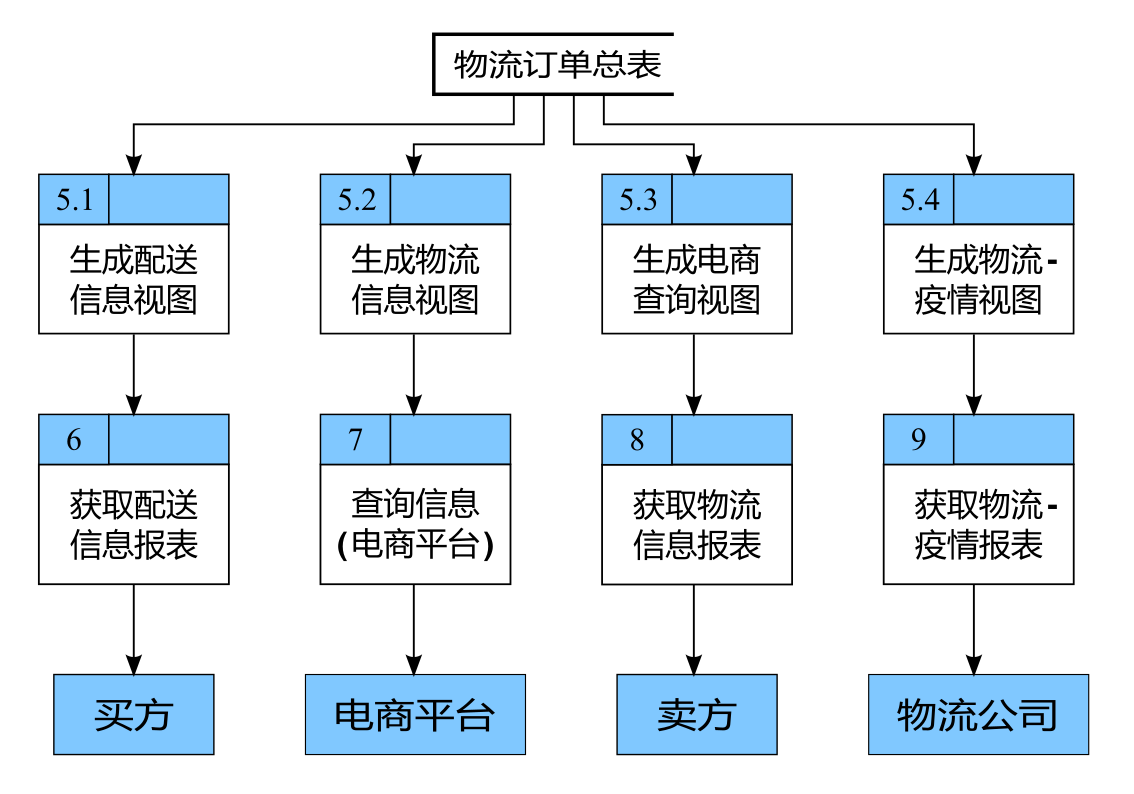
\includegraphics[height = 13cm]{level-2.2.png}
\end{center}

\noindent \textbf{(3) 识别物流风险}
\begin{center}
	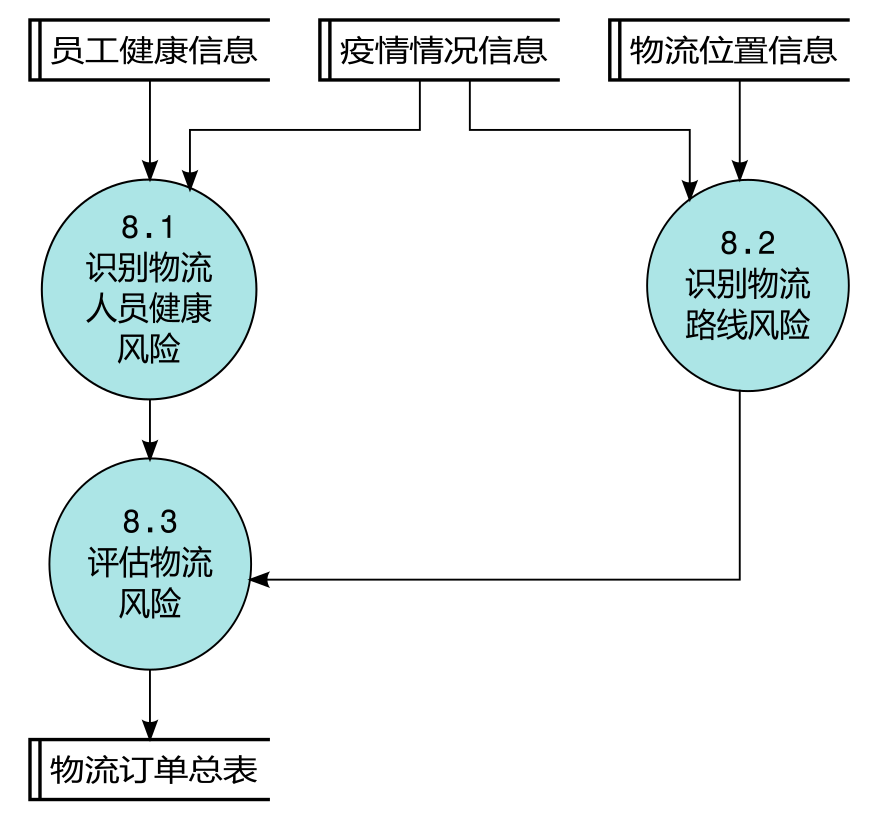
\includegraphics[height = 8cm]{level-2.3.png}
\end{center}

\subsection{数据字典}

\subsubsection{数据项}

\tablehead{
	\toprule
	\textbf{编号} & \textbf{数据项名} & \textbf{含义说明} & \textbf{数据类型} & \textbf{长度} & \textbf{备注} \\
	\midrule}
\tabletail{\bottomrule}

\begin{center}
\begin{supertabular}{llllll}
	1 &	Uname &	买方名称 &	Char &	30 &	非空 \\
	2 &	Uno &	买方编号 &	Integer & 4 &	非空 ,买方用户信  \\ &&&&& 息表主码\\
	3 &	Uaddress &	买方地址 &	Char &	30 &	非空 \\
	4 &	Uphone &	买方联系方式 &	Integer &	4 &	非空 \\
	5 &	Sname &	卖方名称 &	Char &	30 	& 非空\\
	6 &	Sno &	卖方编号 &	Integer &	4 	& 非空,卖方用户信 \\ &&&&& 息表主码 \\
	7 &	Saddress &	卖方仓储位置 &	Char &	30 	& 非空 \\
	8 &	Pname &	配送人员姓名 &	Char &	30 &	非空 \\
	9 &	Pno &	配送人员编号 &	Integer &	4 &	非空 \\
	10 &	Pcity &	人员今日途经城市 &	Char &	30 & 非空 \\
	11  &	Ptemp &	配送人员体温 &	Float &	4 &	非空 \\
	12 &	Pupdate &	健康信息更新时间 &	Date &	3 &	非空 \\
	13 &	Ono &	商品订单编号 &	Integer &	4 &	非空,商品订单信 \\ &&&&& 息表主码\\
	14 &	Otime &	商品订单时间 &	Date &	3 &	非空 \\
	15 &	Iname 	& 货品名称 &	Char &	30 &	非空 \\
	16 &	Ino &	货品编号 &	Integer &	4 &	非空 \\
	17 &	Inum &	订单货品数额 &	Integer &	4 &	非空 \\
	18 &	Tname &	物流公司名称 &	Char &	30 	& 非空 \\
	19 &	Tno &	物流公司编号 &	 Integer &	4 &	非空 \\
	20 &	Ovalue 	& 商品订单金额 	& Float &	4 &	非空 \\
	21 & Dno &	物流单号 &	Integer &	4 &	非空,物流订单信 \\ &&&&& 息表主码 \\
	22 &	Dtrans &	物流运送方式 &	Char &	30 &	非空 \\
	23 &	Dloc &	物流所在位置 &	Integer &	4 &	非空 \\
	24 &	Dupdate &	物流更新时间 &	Date &	3 &	非空 \\
	25 &	Dstate &	物流风险信息 &	Tinyint &	1 &	非空,0异常; \\ &&&&& 1正常\\
	26 &	Cname &	城市名称 &	Char &	30 	& 非空 \\
	27 &	Cno &	城市编号 &	Integer &	4 &	非空 \\
	28 &	Cstate &	城市疫情状况 &	Tinyint &	1 &	 非空,0、1、2分\\ &&&&& 别代表低中高风险 \\
	29 &	Cloc &	城市坐标 &	Float &	4 &	非空 \\
	30 &	Cupdate &	城市疫情更新时间 &	Date &	3 &	非空 \\
	31 &	Dvalue 	& 物流订单金额 	& Float &	4 &	非空 \\
	32 &	Zpeople & 配送人员风险评分 & Integer & 4 & 非空 \\
	33 &	Zloc & 配送路线风险评分 & Integer & 4 & 非空 \\
\end{supertabular}
\end{center}

\newpage
\subsubsection{数据结构}

注:\underline{下划线}表示主码,\textit{斜体}表示外码。

\tablehead{
	\toprule
	\textbf{编号} & \textbf{数据结构} & \textbf{含义说明} & \multicolumn{3}{l}{\textbf{组成}} \\
	\midrule}
\tabletail{\bottomrule}

\begin{center}
\begin{supertabular}{llllll}
1 &	Buyer User &	买方用户信息表 & Uname &	\underline{Uno} &	Uaddress  \\ & Information &&	Uphone && \\
2 &	Seller User &	卖方用户信息表 & Sname &	\underline{Sno} &	Saddress \\ & Information &&&& \\
3 &	Order  & 商品订单信息表 &	\underline{Ono} &	Otime &	Ovalue  \\
& Information &&	Otrans & \textit{Uno} &	\textit{Sno}  \\
4 &	Delivery &	物流订单信息表 &	\underline{Dno} &	Dvalue &	Dtrans  \\ & Information && Tno &	Pno & \textit{Sno} \\
5 &	Staff Health &	员工健康信息表 &	\underline{Pno} &	Pcity & Ptemp \\ 
& Information && \underline{Pupdate} && \\
6 &	Pandemic &	疫情情况信息表 &	Cname &	\underline{Cno} &	Cstate \\	& Information &&  Cloc & \underline{Cupdate}	& \\
7 &Staff  &	物流人员信息表 &	Pname &	\underline{Pno} &	Tname \\ & Information	& & Tno && \\
8 &	Geographic  &	物流位置信息表 &	\underline{Dno} &	Dloc &	\underline{Dupdate} \\& Information&&&& \\
9 & Summary & 物流订单总表 & \underline{Ono} & \textit{Dno} & Zpeople \\ & Information && Zloc && \\
\end{supertabular}
\end{center}

\subsubsection{数据流}

\tablehead{
	\toprule
	\textbf{编号} & \textbf{数据流名} & \textbf{来源} & \textbf{去向} &  \textbf{组成} \\
	\midrule}
\tabletail{\bottomrule}

\begin{center}
\begin{supertabular}{lllll}
	1 & 买方用户信息 &	电商数据同步 &	数据统计 &	买方姓名,联系方式地址等 \\&&& 与可视化 & \\
	2 &	卖方用户信息 & 电商数据同步 &	数据统计 &	卖方姓名,联系方式地址等\\&&& 与可视化 & \\
	3 &	商品订单信息 & 交易 &	提交物流 &	商品订单号,商品名称、 \\ &&&订单& 数量、金额等 \\
	4 &	疫情情况信息 &	官方数据爬取	& 识别物流 &	全国各地区疫情风险情况 \\ &&& 风险 & (每日更新)\\
	5 &	员工健康信息 &	自测健康状况 &	安排配送、 &	员工体温等健康信息 \\ &&& 识别物流 &(每日更新)\\ &&& 风险 &\\
	6 &	物流人员信息 &	公司数据同步 &	安排配送 &	员工编号、姓名等信息 \\
	7 &	物流订单信息 &	提交物流订单	& 安排配送 & 	物流订单号,物流运送方\\ &&&& 式,运费等信息 \\
	8 &	物流位置信息 & 安排配送 &	识别物流 &	物流当前所在位置及所经 \\ &&& 风险 & 过的路径信息 \\
	9 & 物流订单总表 & 识别物流风险 & 数据统计 & 物流疫情相关信息汇总 \\ &&  & 与可视化 & \\
\end{supertabular}
\end{center}

\subsubsection{数据储存}

\tablehead{
	\toprule
	\textbf{编号} & \textbf{数据存储名} & \textbf{输入} & \textbf{输出} &  \textbf{说明} \\
	\midrule}
\tabletail{\bottomrule}

\begin{center}
\begin{supertabular}{lllll}
	1 &	买方用户信息表 &	买家用户信息 	& 无 &	存储所有买家用户信息 \\
	2 &	卖方用户信息表 &	卖家用户信息 &	无 &	存储所有卖家用户信息 \\
	3 &	商品订单信息表 &	商品订单信 &	订单信息 &	存储所有商品订单相关 \\ && 息,价格 && 信息 \\ 
	4 &	物流订单信息表 &	物流信息价 &	物流信息 &	存储所有物流订单的相 \\ && 格,运输方式 && 关信息 \\
	5 &	员工健康信息表 &	配送人员信 &	健康状况 &	存储配送人员每日更新 \\ && 息,健康状况 && 的健康状况信息 \\
	6 &	疫情情况信息表 &	每日国内疫 &	疫情情况 &	存储国内各地区每日疫 \\ && 情情况 & 可视化 & 情情况更新的信息 \\
	7 &	物流人员信息表 &	员工名单 &	无 &	存储物流公司配送人员 \\ &&&& 名单 \\
	8 & 物流位置信息表 &	定时更新物 &	物流路线 &	存储物流位置实时信息 \\ && 流位置坐标 & 可视化 & \\
	9 & 物流订单总表 & 物流单号,& 数据统计 & 存储物流与订单关系\\ && 订单编号 & 与可视化 & \\
\end{supertabular}
\end{center}

\subsubsection{处理过程}

\tablehead{
	\toprule
	\textbf{编号} & \textbf{处理过程名} & \textbf{输入数据流} & \textbf{输出数据流 } &  \textbf{加工逻辑} \\
	\midrule}
\tabletail{\bottomrule}

\begin{center}
\begin{supertabular}{lllll}
	1 &	买方上传信息 &	买方用户信息	& 买方信息查询 &	由买方授权,从电商 \\ &&&& 平台接口进行导入 \\
	2 &	卖方上传信息 &	卖方用户信息 &	卖方信息查询 & 由卖方授权,从电商 \\ &&&& 平台接口进行导入 \\
	3 &	电商平台上传 &	商品订单信息 &	订单查询 &	由电商平台上传订单 \\ & 信息 &&& 信息与买卖关系 \\
	4 & 物流公司上传 & 物流订单信息  &	物流查询  &	由物流公司上传物流 \\ & 信息1 &&& 信息及卖方信息 \\
	5 &	物流公司上传 &	物流人员信息 &	物流查询、物 &	由物流公司进行统计 \\ & 信息2 & & 流人员查询 & 上传 \\
	6 &	配送人员上传 &	每日健康状况 &	配送人员健康 &	由配送人员每日上传 \\ & 信息 & 信息 & 信息 & 当日健康状况信息 \\
	7 &	配送人员健康 &	申请查询配送 &	配送人员健康 &	根据配送人员每日健 \\ & 状况查询 & 人员健康信息 & 信息 & 康状况的统计数据,\\ &&&& 进行查询,检查配送 \\ &&&& 人员健康自检是否满 \\ &&&& 足要求 \\
	8 &	疫情统计 &	爬取城市地区 &	疫情统计可视 &	爬取官方发布的疫情 \\ && 疫情分布情况 & 化结果 & 分布情况,分析地理 \\ && 及坐标 && 位置坐标标注 \\
	9 &	路线查询 &	查询订单坐标 &	坐标路径可视 &	根据物流坐标的信 \\ && 信息 & 化结果 & 息,生成物流路径供 \\ &&&& 买方查看配送进度 \\
	10 &	物流疫情情况 &	路径可视化结 & 疫情-物流图 &	根据疫情与物流坐 \\ & 查询 & 果、疫情统计 && 标,合成疫情-物流 \\ && 可视化结果 && 可视化的图像,并对 \\ &&&& 路径疫情情况进行 \\ &&&& 评估 \\
\end{supertabular}
\end{center}

\subsection{安全性和完整性要求}

\subsubsection{安全性要求}

平台系统的使用者主要分为物流公司、电商平台、卖家、买家和游客。其中,物流公司、电商平台、卖家和买家在使用平台服务前,需要经过注册成为系统用户,在数据库内储存其设置的用户信息,并通过系统核实认证身份,保证身份不被盗用,以确保用户信息的真实性和数据安全性。未经系统核实认证身份的游客只行使浏览权限,且只能够浏览平台提供服务介绍信息和中高风险地区总地图等相关信息。游客无需向系统输入会保留在数据库中的内容,也无法查询超出其游客权限的内容。

由于系统涉及个人隐私数据(如买家卖家基本信息等)和商业敏感性数据(如订单信息,商家成本收益等),为了保护各方隐私安全,系统对于不同的认证用户身份设置了不同的访问权限。对于物流公司身份用户,只能够查看由其提供的物流人员健康信息、包裹配送信息进行数据统计与可视化之后的报告,并对相应信息进行查询;电商平台身份用户只能够查看由其提供订单信息进行数据处理与可视化之后的报告,并进行相应查询;买家用户和卖家用户的个人隐私数据只有本人有权限查看,且只能查询和本人相关的订单及产品包裹配送信息;游客没有任何查询个人隐私数据和商业敏感数据的权限。对于不涉及系统核心业务的数据(如商家成本收益),数据提供者有权选择不提供此类信息。对于任何分析报告中统计性数据,将对涉及订单、用户信息进行匿名化处理,绝不公开个体数据。

\subsubsection{完整性要求}

\noindent \textbf{(1) 实体完整性}
\par
\vspace{0.1cm}
\noindent 作为主码的属性不能取空值且取值唯一,详见数据字典数据项部分的限制条件。

\noindent \textbf{(2) 参照完整性}
\par
\vspace{0.1cm}
\noindent 作为外码的属性或者为空值或者为被参照关系中某个元组的主码值,详见数据字典数据项部分的限制条件。

\noindent \textbf{(3) 用户定义的完整性}
\par
\vspace{0.1cm}
\noindent 根据系统的具体功能,某些属性不能取空值或者对属性的取值范围有限制,详见数据字典数据项部分的限制条件。

\subsection{需求分析过程中的经验教训总结}

随着疫情逐渐常态化,人们对于实时监控周边疫情信息的需求越发迫切。于是,对于作为最容易成为密切接触者,又是人们生活中最常见的物流配送人员的健康状况和包裹近期途径地风险的监控,便成为防控疫情的重中之重。然而,据我们问卷调查显示,在大部分买家看来,现在大多数主流电商平台和物流公司在对物流配送人员和包裹的相关疫情信息监控上所做出的努力还远远不够。信息滞后和防控力度不足亟需社会推出一个新的“疫情+物流”信息整合平台。于是我们组尝试在这方面做出努力,搭建一个能够实现疫情及物流订单数据储存、整合并动态可视化呈现的平台,以同时满足物流公司、电商平台、买家和卖家对于疫情下物流配送及包裹信息的监控需求。由于我们的问卷调查覆盖人群及调研时间有限,问卷所得的结果与实际情况可能存在偏差,这对我们的需求分析可能会造成一定的影响,若时间及条件允许,我们会尝试开展更深入的调查以获得更准确的结论。

\section{概念结构设计}

\subsection{局部分 E-R 图 }

\subsubsection{提交物流订单}

\begin{center}
	
\includegraphics[height = 16cm]{e-r-part-1.png}
\end{center}

\subsubsection{安排配送}

\begin{center}
	
\includegraphics[height = 15.5cm]{e-r-part-2.png}
\end{center}

\subsubsection{识别物流风险}

\begin{center}
	
\includegraphics[height = 17cm]{e-r-part-3.png}
\end{center}

\subsection{全局 E-R 图 }

\subsubsection{不包含属性的 E-R 图}

\begin{center}
	
\includegraphics[height = 16cm]{e-r-total.png}
\end{center}

\subsubsection{每个实体和联系的属性描述}

\noindent \textbf{(1) 卖方}

\begin{center}
	
\includegraphics[height = 3cm]{e-r-e1.png}
\end{center}

\noindent \textbf{(2) 物流公司}

\begin{center}
	
\includegraphics[height = 2.3cm]{e-r-e2.png}
\end{center}

\noindent \textbf{(3) 物流订单}

\begin{center}
	
\includegraphics[height = 10cm]{e-r-e3.png}
\end{center}

\noindent \textbf{(4) 物流人员}

\begin{center}
	
\includegraphics[height = 2.5cm]{e-r-e4.png}
\end{center}


\noindent \textbf{(5) 物流位置}

\begin{center}
	
\includegraphics[height = 2.5cm]{e-r-e5.png}
\end{center}

\newpage
\noindent \textbf{(6) 疫情情况}

\begin{center}
	
\includegraphics[height = 7cm]{e-r-e6.png}
\end{center}

\noindent \textbf{(7) 联系:匹配1}

\begin{center}
	
\includegraphics[height = 1.5cm]{e-r-r1.png}
\end{center}

\noindent \textbf{(8) 联系:匹配2}

\begin{center}
	
\includegraphics[height = 1.5cm]{e-r-r2.png}
\end{center}

\section{逻辑结构设计}

\subsection{E-R 图向关系模型的转换过程}

\subsection{关系模型的优化过程}

\subsection{最终的关系模式}

\subsection{设计用户的子模式}

\section{数据库实施}

\subsection{环境和配置}

\section{相关程序演示}
\section{总结}

\end{document}